\chapter{Mathematical Methods} \label{ch:mathematical-methods}

%\hrulefill
%
%\textbf{Notes on this draft:}
%
%
%The following types of comments are interspersed throughout this working draft. Obviously, these are to be removed by the time of the final draft.
%
%\vtodo{This is a TODO.  Used when something is missing, incomplete, or wrong.
%		These are the most important action items, often requiring additional research or development.
%		For example, ``add example'' or ``derive necessity of gaussian'' i}
% 
%\vcleanup{Lower priority than a TODO. Cleanup-TODOs can and will require in-depth fixes, but it's usually less pressing than a missing/wrong item, which requires a TODO. For example, ``fix transition'' or ``standardize notation'' is a CLEANUP, not a TODO. Roughly, CLEANUPS are for formatting/style concerns, rather than content.}
%
%\vcomment{This is a comment. Used for general remarks about a subject that haven't been merged into the text.
%			These are often descriptions, or suggestions for expansion or deletion of content.}
%
%
%These should be used sparing. Absence of any comment does not indicate that a section is complete or without concerns in any way--these are simply meant to represent ``threads to pull'' in bringing this document closer to completion.

%\hrulefill

Our goal is establish a resource efficient method of finding curvilinear content in 2D grayscale digital images using concepts of differential geometry. We proceed by
\begin{enumerate*}[label=(\roman*)]
	\item establishing a standard method of viewing these images as 2D surfaces,
	\item developing a minimal yet rigorous distillation of differential geometry
			to obtain suitiable quantifiers
			for the study of curvilinear structure in 3D surfaces,
	\item establishing a filter based on these quantifiers,
	and finally
	\item developing methods necessary for efficient computation of the filter.
\end{enumerate*}

%%%%%%%%%%%%%%%%%%%%%%%%%%%%%%%%%%%%%%%%%%%%%%%%%%%%%%%
%%%%%%%%%%%%%%%%%%%%%%%%%%%%%%%%%%%%%%%%%%%%%%%%%%%%%%%
\section{Problem Setup in Image Processing}\label{sec:image-processing-setup}

%\vcomment{This section should be basically describing how to view an image as a surface.
%  Use any notation here that is useful beyond differential geometry, in all the contexts
%  we need to consider the image (in terms of Fourier Theory, scale space theory,
%  Frangi filtering, etc. all together.}

A digital 2D grayscale image is given by a $MxN$ array of pixels, whose intensity is given by an integer value between 0 and 255.

\begin{defn}[Image as a pixel matrix] \label{def:image_as_pixel_matrix}
	\begin{equation*}
	\img \in \N^{M \times N}
	\quad\textrm{with}\quad
	0 \le \img_{ij} \le 2^8 - 1
	\end{equation*}
\end{defn}
	% iI hate this wording.
	For theoretical purposes, we wish to consider any such picture to ultimately be a sampling of a 2D continuous surface. We also require that this surface is sufficiently continuous as to admit the existence of second partial derivatives.
	
\begin{defn}[Image as an interpolated surface] \label{def:image_as_surface}
 \begin{equation*}
 h: \R^2 \to \R
 \quad \textrm{with}\quad
 h \in \mathcal{C}^2\left(\R^2\right),
 \quad\textrm{where}\quad
    h(i,j) = \mathtt{I}_{ij}
    \; \forall (i,j) \in
     \left\{0,...,M\right\} \times
     \left\{0,...,N\right\} \subset \N^2
    \end{equation*}
\end{defn}
% say the same thing with words
That is, the function $h$ is identical to the pixel matrix $\img$ at all integer inputs,
and simply a ``smooth enough'' interpolation of those points for all other values.


It is of course necessary to admit that $\mathtt{I}$ is not really a perfect representation of the underlying ``content'' within the picture. Not only is information lost when $\img$ is stored as an integer, there are also elements of noise and anomalies of lighting that would constitute noise to the original signal. There are multiple treatments of image processing that do address this discrepancy in a pragmatic way \cite{DIPGW}, especially when the goal is noise reduction.
However, we will be content to simply represent the pixels of $\img$ as the ultimate ``cause'' of the surface $h$ in \cref{def:image_as_surface}, and worry not about how faithfully that sampling corresponds to the real world.
% Word salad, also rude? ask chang about this
Moreover, though our samples in the image domain have been carefully prepared (as outlined in \label{sec:NCS-data-set}), there are numerous shortcomings therein, and improvements to the veracity of our original signal could be made from many angles.
Though we shall draw upon the notion of the pixel matrix $\img$ as a sampling again to motivate our development of scale space theory in \cref{sec:scale-space-theory}, we ultimately use these techniques because we find them successful to our problem.
 
%%%%%%%%%%%%%%%%%%%%%%%%%%%%%%%%%%%%%%%%%%%%%%%%%%%%%%%
%%%%%%%%%%%%%%%%%%%%%%%%%%%%%%%%%%%%%%%%%%%%%%%%%%%%%%%
\section{Differential Geometry} \label{sec:differential-geometry}
  
We wish to describe the structure of an image as a surface. To do this, we develop the notion of curvature of a surface in $\R^3$ in a standard way, following \cite{Kuhnel-DiffGeo} (although any undergraduate text in Differential Geometry should prove satisfactory).

\subsection{Preliminaries of Differential Geometry}
%\vcleanup{Mention when you're talking about a general surface in $\R^3$ and when it's specifically a graph and make sure it's clear which case you're dealing with and motivate why you'd want to talk about things that aren't graphs at all (to define shape operator in general). Potentially rework to not talk about non-graphs when irrelevant. Although it's useful to keep some references to non-graphs to align this with "the general picture" and what you'll find in a diff geo textbook, also because I already wasted time doing the hard work.}
    Given an open subset $U\subset \R^2$ and a twice differentiable function  $h: U \to \R$ (as in \cref{def:image_as_surface})
    we define the graph, $f$, of $h$ in the following definition.
    
    \begin{defn} \label{def:graph}
    The surface $f$ is a graph (of the function $h$) when 
    \[
     f: U \to \R^3 \quad \textrm{by} \quad f(u_1, u_2) \;=\; \big(u_1 , u_2 , h(u_1,u_2)\big)
     \;,\quad u = (u_1, u_2) \in U \subset \R^2 \]
    \end{defn}
    %That is, $f$ is an embedding/immersion/parametrization of the function h
    Since the graph $f$ is clearly one-to-one by definition, we may readily associate any input $u\in U$ with
    its corresponding output $p \in f[U]$, i.e.
    $ p = f(u) = f(u_1, u_2) \;=\; \big(u_1 , u_2 , h(u_1,u_2)\big)$,
    % world salad but may need motivation.
    depending on whether we wish to focus on a point of a graph in terms of its input
    or in terms of the structure of the graph itself.
    
    % Motivation
    Our development of curvature ultimately will hinge upon a careful consideration of the tangent plane of $f$ at a point $p$, for we will require a concrete definition of both the tangent space within the domain and image of $f$,
    as well as the so called "differential" of $f$,
    % shit or not because we need it later!
    the lattermost of which we will only define for the immediate case required
    Seeing that $f$ is one-to-one should make a lot of this
    futzing about complete overkill, but I've yet to find a way to distill it. That is, this development works for any parametrized surface element, not necessarily a graph. Whatever for now.
    
    
    \begin{defn}[Tangent space of $U$ at $u$] \label{def:tangent-at-U}
    	\[ T_{u} U = \left\{u\right\} \times \R^2
    	\]
    	\end{defn}
    \begin{defn}[Tangent space of $\R^3$ at $p$]
    	\[ T_{p} \R^3 = \{p\} \times \R^3
    	\]
    \end{defn}
    It is immediately clear that $T_uU$ and $T_p\R^3$ are isomorphic to
    $\R^2$ and $\R^3$, respectively, and we can easily visualize elements of $T_uU$ are tangent vectors in $\R^2$ ``originating'' at the point $u$, and elements of $T_p\R^3$ are tangent vectors ``originating'' at the point $p$.
\begin{defn}[The differential of $f$ at a point $u$] \label{def:differential-map}
       	$Df\vert_u$ is the map from $T_uU$ into $\R^3$ given by
    \[
     Df|_u : T_uU \to T_{f(u)}\R^3
     \quad \textrm{by}
     \quad w \mapsto J_f (u) \cdot v
    \]
where $J_f(u)$ is the Jacobian of $f$ evaluated at some fixed point $u \in U$, i.e. the matrix
\[
J_f (u) = \left[ \left.\frac{\partial f_i}{\partial u_j}\right\vert_u \right]_{i,j}
\]
\end{defn} % You can in some ways argue that J_x(f) is a better notation
Although not necessary presently, we could just as easily consider the differential of an arbitrary function as a map between tangent vectors in the function's domain and tangent vectors in its range.
We could also just identify this as mapping  $U \to \R^3$ by the obvious isomorphism described above. and then differential of $f$ at $x$ is simply a linear transformation of between the tangent spaces $T_uU$ and $T_p\R^3$ where the transformation in question is given by the Jacobian. We can define such a differential at any point $u$ in the domain.

With these three definitions, we are equipped to give a formal definition of $T_uf$,
the tangent plane of $f$ at an input $u$.
\begin{defn}[Tangent plane of a graph]\label{def:tangent-plane}
\[
T_u f := Df\vert_u \left(T_u U\right)
\subset T_{f(u)} \R^3 = T_{p} \R^3
\]
\end{defn}

This vectors of this plane can thus be identified as tangent vectors from $T_uU$ that have been passed through the differential mapping $Df\vert_u$.
We shall denote a generic tangent vector $X \in T_u f$ at point $p$.
%%%%%STOPPEED HERE
We may expand any such vector $X$ in terms of the basis $\left\{ \frac{\partial f}{\partial u_i}\right\}_{i=1,2}$; that is,
$\textrm{span}\left\{ \frac{\partial f}{\partial u_1}, \frac{\partial f}{\partial u_2}\right\} = T_u f$.

% level of "needless" abstraction
Given the level of abstraction above, it may be refreshing to explicitly show the linear independence of this set in the case of an arbitrary graph $f$.
%it's the span though? just say it's the span?
\begin{lemma} \label{lemma:f_ui-is-a-basis}
	When $f$ is a graph, for all points $u \in U$, $\left\{\frac{\partial f}{\partial u_1} , \frac{\partial f}{\partial u_2}\right\}$ is in fact a basis for the tangent plane $T_uf$.
\end{lemma}
Quite obviously, we're assuming $(1,0), (0,1) \in U$. If this is not the case, we pick some $\alpha$ small enough so that $(\alpha,0)$ and $(0,\alpha)$ are contained and this scaled version would serve as a basis instead.
\begin{proof}
Given the definition of a graph $f$ as in \cref{def:graph}, we can directly calculate the partial derivatives of $f$ at a point $u$.
\[
f_{u_1} = (1,0,h_{u_1}(u)) \quad\textrm{and}\quad f_{u_2} = (0,1,h_{u_2}(u))
\]
 which are obviously linearly independent.  Then $Df\vert_u (1,0) = f_{u_1} ,$ and $ Df\vert_u (0,1) = f_{u_2}$, which shows $\left\{\frac{\partial f}{\partial u_1} , \frac{\partial f}{\partial u_2}\right\} \in T_uf$.  Thus $\left\{\frac{\partial f}{\partial u_1} , \frac{\partial f}{\partial u_2}\right\}$ is a linearly independent subset of $T_u f$, and can serve as its basis.\end{proof}

	The partials derivatives of $f$ are not, in general, orthogonal at any point $u$, unless it happens that $h_{u_1} $ or $h_{u_2}$ is zero.
	A visualization of some of the above is given in \cref{fig:Tuf}, although note that $f_{u_1}$ and  $f_{u_2}$ accidentally appear orthogonal.
	
	\begin{figure}\centering
		\includegraphics[width=0.8\textwidth]{T_uf}
		\caption{Tangent plane of a graph}
		\label{fig:Tuf} 
	\end{figure}
%  	But the above allows us to view $Df\vert_u$ differential map of $f$ is exactly the expansion of
%  	a point  $v \in U$ along the basis
%  	$\left\{\frac{\partial f}{\partial u_1} , \frac{\partial f}{\partial u_2}\right\}$ .

We now concern ourselves with developing the notion of curvature on a surface. First, we need to consider an arbitrary regular curve (i.e. differentiable, one-to-one, non-zero derivative) contained within the image of $f$. 
  	
  	% this isn't really a definition...?
 

\subsection{Curvature of a surface and its calculation}
In the context of a regular arc-length parametrized curve $c: I \to \R^3$ parametrized along some closed interval $I\in \R$
 (that is, a differentiable, one-to-one curve where $c'(s) = 1 \;\; \forall s \in I$), curvature at a point $s \in I$ is defined simply as the magnitude of the curve's acceleration: $\kappa(s) := \vnorm{c''(s)}$.
 
 To extend the notion of curvature of a surface $f$, we can consider the curvature of such an arbitrary curve embedded within the surface.
 
 \begin{defn}[Surface curve] \label{def:curve-on-a-surface}
 	Given a closed interval $I \subset \R$, we call the regular curve
 	$c: I \to \R^3$ a surface curve in the event that $\image(c) \subset \image(f)$ entirely. The one-to-one-ness of the graph $f$ ensures that we can define (for the given curve) an intermediary parametrization $\theta_c$  so that
 	$ c = f \circ \theta_c $. That is,
 	\[
 	\theta_c : I \to U \; \textrm{by} \; \theta(t) = \big(\theta_1(t), \theta_2(t)\big)
 	\]
 	
 	so that $c(t) = f(\theta_c(t)) \;\forall t\in I,$
 	and $c[I] = f\left[\theta_c[I]\right].$.
 \end{defn}
 Note as well that the velocity of this particular curve lies within $T_u f$. This
 can be seen by an elementary application of chain rule:
 \begin{align}
 -\frac{d c}{dt} &= -\frac{d}{dt}\big[ f(\theta_c(t))\big] \\
 &= -\frac{d}{dt}\big[f(\theta_1(t), \theta_2(t))\big] \\
 &= \theta_1'(t)\left( \frac{\partial f}{\partial u_1} \right) + 
 \theta_2'(t)\left( \frac{\partial f}{\partial u_2} \right) \in T_uf.
 \end{align}
 
 Considering a point $p \in I$ and its associated point $u = \theta_c(p)$, we wish to compare the curvatures of all (regular) surface curves passing through the point $p$ at some particular velocity.
 
 We now present a main result that provides a notion of curvature of a surface.

	\begin{theorem}[Theorem of Meusnier] \label{thm:meusnier}
		Given a point $u \in U $ and a tangent direction $X \in T_u f$,
  any regular curve on the surface $c: I \to \image(f)$ with $p\in I : \theta_c(p) = u$
  where $c'(p) = X$ will have the same curvature.
	\end{theorem}
	
	%\vtodo{provide a visualization of this}
	
	In other words, any two curves on the surface with a common velocity at a given point on the surface will have the same curvature. To prove this, we'll require one final definition.
	\begin{defn}[The Gauss Map] \label{def:gauss-map}
		The Gauss map at a point $p = f(u)$ is the unit normal to the tangent plane
		\[\nu : U \to \R^3 \quad\textrm{by}\quad  \nu(u) :=
		\frac{\frac{\partial f}{\partial u_1} \times \frac{\partial f}{\partial u_2}}
		{\vnorm{\frac{\partial f}{\partial u_1} \times \frac{\partial f}{\partial u_2}}} \]
	\end{defn}
	Each partial above understood to be evaluated at the input $u \in U$; that is, we calculate $\left.\frac{\partial f}{\partial u_i}\right|_u$.
	The existence of the cross product in its definition makes it clear that $\nu \perp \frac{\partial f}{\partial u_i}$ each $i=1,2$. A simple dimensionality argument of $\R^3$ implies that these must exist in $T_uf$. However, we can also show it directly: 
%	\vcomment{at this point if you can prove $\left\{ \frac{\partial \nu}{\partial u_1}, \frac{\partial \nu}{\partial u_2}\right\}$ are linearly independent then do so, or just save for later, in which case don't use derivates at all}
	
	To show that $\left\{\frac{\partial \nu}{\partial u_1} , \frac{\partial \nu}{\partial u_2}\right\} \in T_u f$,
	first note that at any particular $u \in U$,
	$\inner{\nu}{\nu} = 1 \implies \frac{\partial}{\partial u_i} \inner{\nu}{\nu} = 0$,
	and so by chain rule $2\inner{\frac{\partial \nu}{\partial u_i}}{\nu} = 0
	\implies \frac{\partial \nu}{\partial u_i} \perp \nu $.
	Since $ \nu \perp \spn\left\{\frac{\partial f}{\partial u_i}\right\} $ as well (since $\nu$ its outer product), in  $\R^3$, this implies
	$\spn\left\{\frac{\partial \nu}{\partial u_i}\right\} \parallel
	\spn\left\{\frac{\partial f}{\partial u_i}\right\}$.
	
	Thus, we have $\textrm{span}\left\{ \frac{\partial \nu}{\partial u_1}, \frac{\partial \nu}{\partial u_2}\right\} \subset T_u f$ as well and we can also use it as a basis.
	
	
	We are finally ready to prove \cref{thm:meusnier}, the Theorem of Meusnier.
	
	%%% START HERE %%%%%%
	\begin{proof}
	Let $X\in T_u f$ be given and consider some curve where $\frac{\partial c}{\partial t}(u) = X$ where $X \in T_u f$. We wish to decompose the curve's acceleration along the  orthogonal vectors $X$ and
	the Gauss map $\nu = \nu(u_1, u_2) =
		\frac{\frac{\partial f}{\partial u_1} \times \frac{\partial f}{\partial u_2}}
		{\vnorm{\frac{\partial f}{\partial u_1} \times \frac{\partial f}{\partial u_2}}}$ as in \cref{def:gauss-map}.
		Note that $X$ and $\nu$ are indeed orthogonal,
		as $ X \in \spn\left\{\frac{\partial f}{\partial u_i}\right\} = T_u f$, and
		$\nu \perp T_u f$).
	 We then have (at this fixed point $u=\theta_c(p)$)
		
		\begin{equation} \label{eq:meusnier_acceleration}
			c'' = \inner{c''}{X} X + \inner{c''}{\nu}\nu
			\end{equation}. 
	
	Because $c$ is a regular curve, we either have $c''=0$,
	or $c' \perp c''$, since $\vnorm{c'} = 1$ implies
	$0 = \frac{d}{dt} \inner{c'}{c'} = 2 \inner{c''}{c'} $. Thus
	
		\[ \inner{c''}{X} = \inner{c''}{c'} = 0 \]

	
	 and we can rewrite the second coefficient of \cref{eq:meusnier_acceleration} using the chain rule: % prove chain rule?
	\begin{align}
		\inner{c''}{\nu} &=
		\frac{\partial}{\partial t}\left[ \inner{c'}{\nu} \right]
			- \inner{c'}{\frac{\partial \nu}{\partial t}} \\
			&= \frac{\partial}{\partial t}\left[ \inner{X}{\nu} \right]
			- \inner{c'}{\frac{\partial \nu}{\partial t}} \\
			&= 0 - \inner{X}{\frac{\partial \nu}{\partial t}}
			%&= \inner{X}{\wein X} = \mathbf{II}(X,X)
			\end{align}
	
	Thus, we can express the curvature at this point on our selected curve as
	\begin{align}
	%\vnorm{c''} = \mathbf{II}(X,X) \vnorm{\nu} = \mathbf{II}(X,X)
	\vnorm{c''} = \vnorm{\inner{c''}{X} X + \inner{c''}{\nu}\nu}
	&= \vnorm{0 + \inner{c''}{\nu}\nu} \\
	&= - \inner{X}{\frac{\partial \nu}{\partial t}}\vnorm{\nu} \\
	&= - \inner{X}{\frac{\partial \nu}{\partial t}} \\
	&=  \inner{X}{-\frac{\partial \nu}{\partial t}} \label{eq:expand_accel_norm}
	\end{align}
	
	We may compute the quantity $-\frac{\partial \nu}{\partial t}$ that appears in
	\cref{eq:expand_accel_norm} via chain rule:
	\begin{align} \label{gaussmap_timederivative}
	-\frac{d \nu}{dt} &= -\frac{d}{dt}\big[\nu(u_1, u_2)\big] \\
	&= -\frac{d}{dt}\big[\nu(\theta_1(t), \theta_2(t))\big] \\
	&= \theta_1'(t)\left( - \frac{\partial \nu}{\partial u_1} \right) + 
	\theta_2'(t)\left( - \frac{\partial \nu}{\partial u_2} \right) \label{eq:gaussmap_dt_expanded}
	\end{align}
	
	
	Identifying $\textrm{span}\left\{ - \frac{\partial \nu}{\partial u_i}\right\}_{i=1,2}$ as a subset of $T_u f$,  we can define a linear transformation $\wein$ which maps the basis
	$\left\{ \frac{\partial f}{\partial u_i}\right\}_{i=1,2}$ to this subset:
	
	\begin{defn}[The Weingarten Map] \label{def:wein-map}
		\[
		\wein: T_u f \to T_u f 
		\quad \textrm{given by the composition} \quad
		\wein = D\nu \circ (Df)^{-1}.
		%\wein(\frac{\partial f}{\partial u_i})
		%	= - \frac{\partial \nu}{\partial u_i}
		%\quad i=1,2		
		\]
	\end{defn}
	That is, $\wein(\frac{\partial f}{\partial u_i}) = - \frac{\partial \nu}{\partial u_i} $ for $i=1,2$, where the negative sign comes about from blind adherence to \cref{eq:gaussmap_dt_expanded} and \cref{eq:expand_accel_norm}. We will This allows us to rewrite the time derivative of the Gauss map \cref{gaussmap_timederivative} as
		\begin{align}
		-\frac{d \nu}{dt} &= 
		\theta_1'(t)\left( - \frac{\partial \nu}{\partial u_1} \right) + 
		\theta_2'(t)\left( - \frac{\partial \nu}{\partial u_2} \right) \\
		&= \theta_1'(t)\left( \wein\left(\frac{\partial f}{\partial u_1}\right) \right) + 
		\theta_2'(t)\left( \wein\left(\frac{\partial f}{\partial u_2}\right) \right) \\
		&= \wein\left[\theta_1'(t)\left( \frac{\partial f}{\partial u_1}\right)  + 
		\theta_2'(t)\left( \frac{\partial f}{\partial u_2} \right)\right] \\
		&= \wein\left(\frac{d}{dt}\left[ f\left(\theta(t)\right)\right] \right)
		= \wein\left( \frac{d}{dt} \left[ c(t) \right] \right) = \wein\left(X\right)
		\end{align} 
		With this, we can re-express the curvature of our curve from
		\cref{eq:expand_accel_norm} as the much simpler
		
		\begin{equation} \label{eq:expand_accel_norm_final}
		\vnorm{c''} = \inner{X}{-\frac{\partial \nu}{\partial t}} = \inner{X}{\wein(X)}
		\end{equation}
		
	
	The linear transformation $\wein$ from \cref{def:wein-map}, and thereby
	the computation of curvature given in \cref{eq:expand_accel_norm_final},
	depends only on the point $u$ and the selected direction $X$, not on the particular curve $c$ at all.
	\end{proof}
	To recap, given a point $u$ on the surface and an arbitrary vector $X$ in the tangent plane, we can calculate the curvature of any surface curve with velocity $X$ there. In fact, we refer to this intrinsic quantity as the normal curvature of the surface.
	
	\begin{defn} \label{def:normal-curvature}
		The normal curvature of a surface, denoted $\kappa_\nu$ at point $u$ in the direction $X$ is given by
		\[\kappa_\nu :=  \inner{X}{\wein(X)} \]
	\end{defn}
	In fact, \cref{thm:meusnier} shows that the normal curvature is an intrinsic property of the surface--it depends only on the
	surface at a point, and no reference to any particular curve on the surface is necessary or implied.
%	In other contexts (not necessary here), this quantity is referred to as the \textit{second fundamental form} at the point $u \in U$; that is, $ \mathbf{II}(X,X) := \inner{X}{\wein(X)}$.
	
	
	The map $\wein$ introduced in the proof above is known as the Weingarten map
	and is implicitly defined at each $u \in U$. 
	We wish to make its existence rigorous as well as find a matrix representation for it, using the standard motivation that $\wein(\frac{\partial f}{\partial u_i}) = - \frac{\partial \nu}{\partial u_i}$.
	
	
	That is, we may trace any $X \in T_u f$ which has been expanded in terms of the basis 
	$\left\{\frac{\partial f}{\partial u_1} , \frac{\partial f}{\partial u_2}\right\}$
	and map it to the span of $\left\{-\frac{\partial \nu}{\partial u_1} , -\frac{\partial \nu}{\partial u_2}\right\}$. 
	
	The Weingarten map can be formally shown to be well-defined, invariant under coordinate transformation in the general case, which is certainly useful for surfaces $f$ that are not graphs. We refer to \cite{Kuhnel-DiffGeo} for the general proof. The situation is much less delicate if $f$ is a graph--the linear transformation may be simply constructed, and we proceed by simply calculating its matrix representation.	
	\begin{lemma}
		The Weingarten map as in \cref{def:wein-map} is well-defined for graphs.
	\end{lemma}
	To find a matrix representation for $\wein$, (which we will denote $\weinmat \in R^{2\times2}$) we simply wish to find a linear transformation
	such that
	$\weinmat \left.\frac{\partial f}{\partial u_i}\right|_{T_u f}
		= - \left.\frac{\partial \nu}{\partial u_i}\right|_{T_u f} \quad \textrm{for} \; i=1,2$
			where $- \left.X\right|_{T_u f}$ denotes that $X \in T_u f$ is being represented in so-called
	'local coordinates' for $T_u f$ (Strictly speaking, of course $T_u f \subset \R^3$ and thus
	$\frac{\partial f}{\partial u_i} \in \R^3.$ Thus when we say $ \left.\frac{\partial f}{\partial u_i}\right|_{T_u f}$ we are referring to this 3-vector expanded with respect to the two-dimensional basis for $T_u f$). In matrix form, we describe this situation as
	
	\begin{align}
	\Bigg[ \;\weinmat\; \Bigg]
	\left[ \mcol{\left.\frac{\partial f}{\partial u_1}\right|_{T_u f}} \;
			\mcol{\left.\frac{\partial f}{\partial u_2}\right|_{T_u f}} \right]
			&= \left[ \weinmat \mcol{\left.\frac{\partial f}{\partial u_1}\right|_{T_u f}} \;
			\weinmat \mcol{\left.\frac{\partial f}{\partial u_2}\right|_{T_u f}} \right] \\
			&= \left[ \mcol{ \left.-\frac{\partial \nu}{\partial u_1}\right|_{T_u f}} \;
			\mcol{\left.-\frac{\partial \nu}{\partial u_2}\right|_{T_u f}} \right]
			\end{align}
			Now, representing each vector in  $T_u f$ with respect to the basis $\left\{ \frac{\partial f}{\partial u_i}\right\}$, we have
			\begin{align}
			\implies
			\Bigg[ \;\weinmat\; \Bigg]
			\begin{bmatrix} - \frac{\partial f}{\partial u_1} - \\
				- \frac{\partial f}{\partial u_2} -
							\end{bmatrix}
			\left[ \mcol{\frac{\partial f}{\partial u_1}} \;
				\mcol{\frac{\partial f}{\partial u_2}}\right]
				&= \begin{bmatrix} - \frac{\partial f}{\partial u_1} - \\
				- \frac{\partial f}{\partial u_2} -
				\end{bmatrix}
				\left[ \mcol{-\frac{\partial \nu}{\partial u_1}} \;
				\mcol{-\frac{\partial \nu}{\partial u_2}}\right]
	\end{align}
		 
	We can simplify this greatly by defining 
	\begin{equation}\label{fundamentalformcoefficients}
	g_{ij} := \inner{\frac{\partial f}{\partial u_i}}{\frac{\partial f}{\partial u_j}}
	\quad \textrm{and}\quad
	h_{ij} := \inner{\frac{\partial f}{\partial u_i}}{-\frac{\partial \nu}{\partial u_j}}
	\end{equation}
	
	so that
	\begin{equation}
	\Bigg[ \;\weinmat\; \Bigg]
	\begin{bmatrix} g_{11} & g_{12} \\ g_{21} & g_{22} \end{bmatrix}
	= \begin{bmatrix} h_{11} & h_{12} \\ h_{21} & h_{22} \end{bmatrix}
	\end{equation}
	
	Then we rearrange to solve for $\weinmat$ as
		\begin{equation} \label{weinmatconstruction}
		\weinmat
		\;=\; \begin{bmatrix} h_{11} & h_{12} \\ h_{21} & h_{22} \end{bmatrix}
		\left.\begin{bmatrix} g_{11} & g_{12} \\ g_{21} & g_{22} \end{bmatrix}\right.^{-1}
		\end{equation}
	
	where $\left[ g_{ij} \right]$ is clearly invertible, as the set
	$\left\{\frac{\partial f}{\partial u_j}\right\}$ is linearly independent.
	
	It should be noted that this matrix representation is accurate not only for the surface of a graph, but for any \textit{generalized} surface
	$f: U \to \R^3 $ with $u \mapsto (x(u), y(u), z(u))$ as well. We shall later show that this calculation simplifies (somewhat) in the case that our surface is a graph.
	
	
	Our final goal to is to characterize such normal curvatures.
	Namely, we wish to establish a method of determining in which directions an extremal normal curvature occurs.
	
	
	\subsection{Principal Curvatures and Principal Directions}
	To do so, we shall consider the relationship between the direction $X$ and the normal curvature $\kappa_\nu$ in that direction at some specified $u$.


	
	First, we need the following lemma:
    \begin{lemma}
        If $A\in R^{n\times n}$ is a symmetric real matrix, $v \in R^n$
        and given the dot product $\inner{\cdot}{\cdot}$,
        we have $\nabla_{v} \inner{v}{Av} = 2Av$.
        In particular, when $A = I$ the identity matrix, we have
        $ \nabla_{v} \inner{v}{v} = 2v$.
    \end{lemma}
    
    \begin{proof}
        The result is uninterestingly obtained by tracking
        each (the `$i$th') component of
        $\nabla_{v} \inner{v}{Av}$:
        
        \begin{align}
        {\Big(\nabla_{v} \inner{v}{Av}\Big)}_{i} =
                \frac{\partial}{\partial v_i} \Big[
                \inner{v}{Av}\Big]
                &=  \frac{\partial}{\partial v_i} \left[
                    \sum_{j=1}^{n} v_j {(Av)}_j\right] \\
                &=	\frac{\partial}{\partial v_i} \left[
                \sum_{j=1}^{n} v_j \sum_{k=1}^n a_{jk} v_k \right] \\
                &= \frac{\partial}{\partial v_i} \left[
                a_{ii} v_i^2 + v_i \sum_{k\ne i} a_{ik} v_k
                 + v_i \sum_{j\ne i} a_{ji} v_j
                 + \sum_{j\ne i} \sum_{k \ne i} v_j a_{jk} v_k \right] \\
    &=  2 a_{ii} v_i + \sum_{k\ne i} a_{ik} v_k
    + \sum_{j\ne i} a_{ji} v_j + 0 \\
    &= 2 a_{ii} v_i + 2 \sum_{k\ne i} a_{ik} v_k
     = 2 \sum_{k=1}^n a_{ik}v_{k} = 2 {\big(Av\big)}_i \\
     &\quad \implies \nabla_{v} \inner{v}{Av} = 2Av.
        \end{align}
    \end{proof}
    
    We are now ready for the major result of this section, which ties the Weingarten map to the
    notion of normal curvatures.
    
    \begin{theorem}[Theorem of Olinde Rodrigues]
       	Fixing a point $u \in U$, a direction $X \in T_u f $ minimizes the normal curvature $\kappa_\nu = \inner{\wein X}{X}$ subject to $\inner{X}{X}= 1$
       	iff $X$ is a (normalized) eigenvector of the Weingarten map $\wein$.
       	\end{theorem}
    \begin{proof}
       	%	Recall first the definition of the first two fundamental forms,
       		%$\textbf{II}(X,X) = \inner{\wein{X}}{X}$
       	%	and $\textbf{I}(X,X) = \inner{X}{X}$.
       		
       		In the following, we will assume that $X \in T_u f$ is expanded,
       		in local coordinates, i.e. along  a two dimensional basis
       		(such as $\left\{ \frac{\partial f}{\partial u_i}\right\}_{i=1,2}$
       		) and thus can refer to $\wein$ freely as the $2\times2$ matrix $\weinmat$.
       		Using the method of Lagrange multipliers, we define the Lagrangian:
       		\begin{equation}
       		\mathscr{L}(X; \lambda) :=
        	\inner{\weinmat X}{X} - \lambda\Big(\inner{X}{X} - 1\Big) 
     \end{equation}
        	
        	Extremal values occur when
        	$\nabla_{X,\lambda} \mathscr{L}(X;\lambda) = 0$,
        	which results in the two equations
        	
     \begin{equation} \label{lagrange_requirements}
     \left\{ \begin{aligned}
      \nabla_X \inner{\weinmat X}{X} - \lambda \nabla_X \left( \inner{X}{X} - 1 \right) = 0 \\
      \inner{X}{X} - 1 = 0
     \end{aligned} \right.
     \end{equation}
     
     The second requirement is simply the constraint that $X$ is normalized.
     Using the previous lemma, we can simplify the first result as follows:
     
     \begin{gather}
     \nabla_X \inner{\weinmat X}{X} - \lambda \nabla_X \left( \inner{X}{X} - 1 \right) = 0 
     \nonumber \\
     2\weinmat X - \lambda \left(2 X \right) = 0  \nonumber \\
     \implies \quad \weinmat X - \lambda X = 0 \nonumber \\
     \implies \quad \weinmat X = \lambda X
     \end{gather}
     which implies that $X$ is an eigenvector of  $\weinmat$ with corresponding eigenvalue $\lambda$ ($X\ne 0 $ from the second equation of \cref{lagrange_requirements}).
     Thus the two hypotheses are exactly equivalent when $X$ is normalized. It is also worth remarking that the corresponding eigenvalue $\lambda$ is the Lagrangian multiplier itself.
       	\end{proof}
       	
       	Thus, to find the directions of greatest and least curvature of a surface at a point $u \in U$, we simply must calculate the Weingarten map and its eigenvectors. We refer to these directions as follows.
       	
       	\begin{defn}[Principal Curvatures and Principal Directions]
       		The extremal values of normal curvature of a surface at a point  $u\in U$
       		are referred to as \textbf{principal curvatures}. The corresponding directions at which normal curvature attains an extremal value are referred to as \textbf{principal directions}.
       	\end{defn}
       	
       	Our final goal is to explicitly determine a (hopefully simplified) version of the Weingarten map in the case of a graph $f(u_1,u_2) = (u_1,u_2, h(u_1,u_2))$ and calculate
       	the principal directions and curvatures in a simple example.
       	        		
       	\begin{theorem}[Relationship between Hessian and Weingarten Map of a Graph]
        	Given the graph $f: U \to \R^3$ where $(x,y) \mapsto (x, y, h(x,y))$, the matrix
        	representation of its Weingarten map is given by
        	\begin{equation} \label{weinmatexactgraph}
        	\weinmat = \Hess(h) \tilde{G} \;,\quad \mathrm{where} \quad
	        	\tilde{G} := \frac{1}{\sqrt{1+h_x^2 + h_y^2}}
	        	\begin{bmatrix}
		        	1 + h_y^2 & -h_x h_y \\
		        	-h_x h_y & 1 + h_x^2 \\
	        	\end{bmatrix} 
        	\end{equation}
        	
        	In particular, given a point $u = (x,y) \in U \subset \R^2$ where $h_x \approx h_y \approx 0$, we
        	have $\tilde{G} \approx \mathrm{Id}$, and thus $\weinmat \approx \Hess(h)$.
        	
       	\end{theorem}
       	\begin{proof}
       		First, we can (using chain rule) rewrite each component as in  \cref{fundamentalformcoefficients}:
      		 \[ h_{ij} = \inner{\frac{\partial f}{\partial u_i}}{-\frac{\partial \nu}{\partial u_j}}
       		= \inner{\frac{\partial^2 f}{\partial u_i \partial u_j}}{\nu} \]
       		
       		Now, given our particular surface $f$, we can calculate each of these components directly. We have:
       		\begin{equation}
       		\begin{gathered}
       		f_{x} = (1, 0, h_x) , \quad
       		f_{y} = (0, 1, h_y)  \\
       		f_{xx} = (0, 0, h_{xx}) , \quad
       		f_{xy} = (0, 0, h_{xy}) = f_{yx} , \quad
       		f_{yy} = (0, 0, h_{yy})
       		\end{gathered}
       		\end{equation}
       		
       		and we have the unit normal vector (Gauss map)
       		\begin{align}
       		\nu(u_1, u_2) &=
       		\frac{\frac{\partial f}{\partial x} \times \frac{\partial f}{\partial y}}
       		{\vnorm{\frac{\partial f}{\partial x} \times \frac{\partial f}{\partial y}}} \\
       		&= \frac{(1, 0, h_x) \times (0, 1, h_y)}{\vnorm{(1, 0, h_x) \times (0, 1, h_y)}} \\
       		&= \frac{\left( -h_x , -h_y , 1 \right)}{\sqrt{h_x^2 + h_y^2 + 1}}
	 \end{align}
	 We then calculate each $h_{ij}$ as
	 \begin{equation}
	 \begin{gathered}
	 h_{11} = \inner{\frac{\partial^2 f}{\partial x^2}}{\nu} = 
		 \frac{h_{xx}}{\sqrt{1+h_x^2 + h_y^2}} \\
	  h_{12} = \inner{\frac{\partial^2 f}{\partial x \partial y}}{\nu} = 
	  \frac{h_{xy}}{\sqrt{1+h_x^2 + h_y^2}} = h_{21} \\
	  h_{22} = \inner{\frac{\partial^2 f}{\partial y^2}}{\nu} = 
	  \frac{h_{yy}}{\sqrt{1+h_x^2 + h_y^2}} \\
	 \end{gathered}
	 \end{equation}
	 
	 and thus the first matrix in \cref{weinmatconstruction} is given by
	 
	 \begin{equation} \label{hij_exactgraph}
	 [h_{ij}] = \frac{1}{\sqrt{1+h_x^2 + h_y^2}} \,  \Hess (h)
	 \end{equation}
	 
	 To calcuate the second, we use
	 
	 
	 
	 \begin{equation}
	 \begin{gathered}
	 g_{ij} = \inner{\frac{\partial f}{\partial u_i}}{\frac{\partial f}{\partial u_j}} \\
	 g_{11} = \inner{f_x}{f_x} = 1 + h_x^2 \\
	 g_{12} = \inner{f_x}{f_y} = h_x h_y = g_{21} \\
	 g_{22} = \inner{f_y}{f_y} = 1 + h_y^2
	 \end{gathered}
	 \end{equation}
	 
	 and thus
		\begin{equation} \label{gij_exactgraph}		 
		[g_{ij}]^{-1} = \begin{bmatrix} 1 + h_x^2 & h_x h_y \\
					h_x h_y & 1 + h_y^2 \end{bmatrix}^{-1}
					\;=\;	\begin{bmatrix} 1 + h_y^2 & -h_x h_y \\
					-	h_x h_y & 1 + h_x^2 \end{bmatrix}
		\end{equation}
       	
       	Combining $[h_{ij}]$ and $[g_{ij}]^{-1}$ from \cref{gij_exactgraph} and \cref{hij_exactgraph}
       	we arrive at \cref{weinmatexactgraph}.
       	\end{proof}
       	
  Thus the matrix of the Weingarten map $\weinmat$ is the Hessian matrix exactly at a critical point $u \in  U$, where $\nabla h(u) = (h_x(u), h_y(u)) = 0$. Of course this implies that $\weinmat$ and $\Hess{(h)}$ have the same eigenvalues and eigenvectors at these points.
  
But this observation is more broadly useful than that, since if $\tilde{G}$ above is close to identity, then the eigenvalues and eigenvectors of $\weinmat$ will be similarly close to the eigenvalues of the Hessian. We can rewrite $\tilde{G}$ from \cref{weinmatexactgraph} as identity plus a small matrix:
\begin{equation}
\tilde{G} = I + [\delta], \quad  [\delta] := \begin{bmatrix} h_y^2 & -h_x h_y \\ -h_x h_y & h_x^2 \end{bmatrix}
\end{equation}

We can then rewrite \cref{weinmatexactgraph} as 
\begin{equation}
\weinmat = \frac{1}{\sqrt{1+h_x^2 + h_y^2}} \Hess(h)
+ \frac{1}{\sqrt{1+h_x^2 + h_y^2}} \Hess(h) [\delta]
\end{equation}

We can see that as $h_x, h_y$ are close to zero, $[\delta]$ will be very close to the zero matrix (and the constant$\frac{1}{\sqrt{1+h_x^2 + h_y^2}}$ will be very close to 1 as well), and we should not expect the addition of a "close to 0" matrix to have much effect on the eigenvectors or eigenvalues. This intuition is confirmed by a result from Wilkinson \cite{wilkinson-eigenvalue}, which we state without rigorous proof.

% see wilkinson pg 66
\begin{theorem}
	If $A$, $B$ are matrices such that $\abs{A_{ij}} < 1 , \abs{B_{ij}} < 1$ (a condition that can be ignored with scaling) and $\lambda$ is a simple eigenvalue of $A$, then given $\epsilon > 0$, there exists a simple eigenvalue $\tilde{\lambda}$ of the matrix $A + \epsilon B$ with $\abs{\lambda - \tilde{\lambda}} = \bigO(\epsilon)$. Similarly, if $v$ is an eigenvector of A, then $\tilde{v}$ is an eigenvector of $A + \epsilon B$ with
	$\abs{v - \tilde{v}} = \bigO(\epsilon)$.
\end{theorem}

The proof ultimately relies on a general result of analysis, that the zeros of a polynomial are continuous with respect to its coefficients. In this case, the polynomial in question is the characteristic polynomial
$p(\lambda) = \det(\lambda I - A - \epsilon B)$, whose coefficients will scale with $\epsilon$. Thus $\weinmat \approx \Hess(h)$ for any point where the gradient $\nabla h \approx 0$. We shall see that we're only concerned with regions where $h_x, h_y$ is small anyway, and we do not expect 

In the event that we do wish to rigorously compute the Weingarten map should want to be rigorously computed "without approximation"--that is, without concern for the magnitude of the gradient--we refer to \cite{jiao2008consistent} and survey papers mentioned therein.

  
  To make the Weingarten map and its relationship to the Hessian more explicit, we will calculate the Weingarten map for a relatively simple graph.
  
  \subsection{The Weingarten map and Principal Curvatures of a Cylindrical Ridge} \label{sec:calculate-weinmap-of-a-ridge}
  
  Let $f$ be the graph given by 
  \begin{equation}
   f: \R^2 \to \R^3 \;\textrm{by}\; f(x,y) = (x,y,h(x,y)), \;\textrm{with}\;
   h(x,y) = \begin{cases}
    \sqrt{r^2 - x^2} & -r \le x \le r \\
    0 & \textrm{else}
    \end{cases}
  \end{equation} 
  \begin{figure}[h!]
  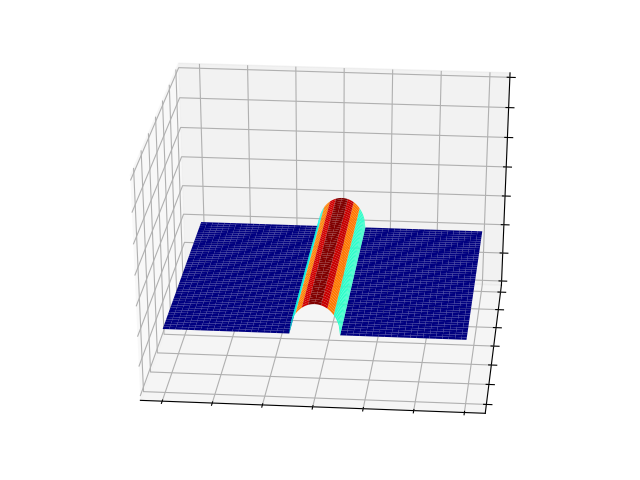
\includegraphics[width=\linewidth]{circular_trough}
  \caption{The graph of a cylindrical ridge of radius $r$}
  \label{fig:ridge-graph}
  \end{figure}
  
  
  The graph is shown in \cref{fig:ridge-graph}. We calculate the necessary partial derivatives of $f$ as follows:
  
  \begin{gather}
  \frac{\partial f}{\partial x} = \left(1, 0, \frac{-x}{\sqrt{r^2 - x^2}}\right)
  \quad , \quad
  \frac{\partial^2 f}{\partial x^2} = \left(0, 0, \frac{-r^2}{\left(\sqrt{r^2 - x^2}\right)^3}\right) \\
  \frac{\partial f}{\partial y} = \left(0, 1, 0\right)
  \quad , \quad
  \frac{\partial^2 f}{\partial y^2} = \frac{\partial^2 f}{\partial x \partial y} = 0
  \end{gather}
  The gauss map is given by
  \begin{gather}
  \nu(x,y) = \frac{\frac{\partial f}{\partial x} \times \frac{\partial f}{\partial y}}
  {\vnorm{\frac{\partial f}{\partial x} \times \frac{\partial f}{\partial y}}}
  = \left( \frac{x}{r} ,\; 0 ,\; \frac{\sqrt{r^2 - x^2}}{r} \right) \\
\implies
\frac{\partial \nu}{\partial x}
 = \left(\frac{1}{r} \;,\; 0\;,\; \frac{-x}{r\sqrt{r^2-x^2}}\right)
 \quad , \quad \frac{\partial \nu}{\partial y} = \left(0,0,0\right).
  \end{gather}
  
  We then calculate matrix elements of the Weingarten map's construction as given in
  \cref{hij_exactgraph} and \cref{gij_exactgraph} :
  \begin{align}
  [h_{ij}] = \frac{1}{\sqrt{1+h_x^2 + h_y^2}} \,  \Hess (h)
     &= \frac{1}{\sqrt{1+\left(\frac{x^2}{r^2-x^2}\right)}}
     \begin{bmatrix}
     \frac{-r^2}{\sqrt{r^2 - x^2}^3} & 0 \\
    0 & 0
     \end{bmatrix} 
     = \begin{bmatrix}
     \frac{-r}{r^2 - x^2} & 0 \\
     0 & 0
     \end{bmatrix} \\
     [g_{ij}]^{-1} &= \begin{bmatrix} \frac{r^2 - x^2}{r^2} & 0 \\ 0 & 1 \end{bmatrix} \\
     \implies \weinmat = [h_{ij}]	[g_{ij}]^{-1} &=
     \begin{bmatrix}
     \frac{-r}{r^2 - x^2} & 0 \\
     0 & 0
     \end{bmatrix} \begin{bmatrix} \frac{r^2 - x^2}{r^2} & 0 \\ 0 & 1 \end{bmatrix} \\
     &= \begin{bmatrix} - \frac{1}{r} & 0 \\ 0 & 0 	\end{bmatrix}	       	
  \end{align}
  
  We see that $u_2 = (0,1)$ and $u_1 = (1,0)$ are eigenvectors for $\weinmat$ with respective eigenvalues
  $\kappa_2 = -\frac{1}{r} , \kappa_1 = 0$. Given the theorem of Olinde Rodriguez suggests that $u_2$ points in the direction of maximum curvature of the surface, $-\frac{1}{r}$, which is predictably in the direction directly perpendicular to the trough, whereas the direction of least curvature is along the trough and is $0$. The theorem of Meusnier \cref{thm:meusnier} suggests that the normal curvature $\kappa_2 = -\frac{1}{r}$ is reasonable-- any curve on the trough perpendicular to the ridge should have the curvature of a circle (the negative simply indicates that we are on the ``outside'' of the surface). Finally, we note that at the ridge of the trough is exactly where $\nabla f = 0$, and the Weingarten map is exactly the Hessian matrix there.
  
  \vcleanup{this was dropped in here. fix the transition}
  Viewing the surface in $\R^3$, we define the Hessian \vcomment{notation here, does it need to be an operator?} $\Hess(x,y)$ of the surface $L$
  at a point $(x,y)$ on the surface as the matrix of its second partial derivatives:
  \begin{equation}
  \Hess(x,y) = \begin{bmatrix}
  L_{xx}(x,y) & L_{xy}(x,y) \\
  L_{yx}(x,y) & L_{yy}(x,y)
  \end{bmatrix}
  \end{equation}
  
  At any point $(x,y)$ we denote the two eigenpairs of $\Hess(x,y)$ as
  \begin{equation}
  \Hess(x,y) u_i = \kappa_i u_i \; , \quad i = 1,2
  \end{equation}
  
\vcleanup{the eigenvectors of the Weingarten map are orthonormal. the eigenvectors of the hessian are also orthonormalizable. make the distinction!}
  where $\kappa_i$ and $u_i$ are known as the
  \textit{principal curvatures} and \textit{principal directions} \vcomment{fixthis} of $L(x,y)$, respectively, and we label such that $|\kappa_2| \ge |\kappa_1|$. Notably, $\Hess(x,y)$ is a real, symmetric matrix (since  $L_{xy} = L_{yx}$ and $L$ is a real function) and thus its eigenvalues are real and its eigenvectors are orthonormal to each other, as given by following basic result from linear algebra,
  \cite{burden-faires}:
  
  % from burden and faires corollary 9.17
  \begin{lemma}[Principal Axis Theorem?]
     	Let $A$ be a real, symmetric matrix. The eigenvalues of $A$ are real and its eigenvectors are orthonormal to each other.
  \end{lemma}
  
  \begin{proof}
     	Let $x\ne 0$ so that $Ax = \lambda x$. Then 
     	\begin{align*}
     	\vnorm{Ax}_2^2 = \inner{Ax}{Ax}  &= (Ax)^{*} Ax \\
     	&= x^{*}A^{*}Ax = x^{*}A^T A x = x*A A x \\
     	&= x^{*} A \lambda x = \lambda x^{*} A x \\
     	&= \lambda x^{*} \lambda x = \lambda^2 x^{*} x = \lambda ^2 \vnorm{x}_2^2
     	\end{align*}
     	Upon rearrangement, we have
     	$\lambda^2 = \frac{\vnorm{Ax}_2^2}{\vnorm{x}_2^2} \ge 0 \implies \lambda $ is real.
     	
     	To prove that a set of orthonormalizable eigenvectors exists,
     	let $A$ be real, symmetric as above and consider the eigenpairs
     	$Av_1 = \lambda_1 v_1$, $Av_2 = \lambda_2 v_2$ with $v_1, v_2 \ne 0$.
     	\footnote{To simplify notation, we simplify our argument to consider two explicit eigenvectors only, since we're only concerned with the $2\times 2$ matrix $\Hess$
     		anyway.}
     	
     	In the case that $\lambda_1 \ne \lambda_2$, we have
     	\begin{align*}
     	(\lambda_1 - \lambda_2)v_1^T v_2 &= \lambda_1 v_1^T v_2 - \lambda_2 v_1^T v_2 \\
     	&= (\lambda_1 v_1)^T v_2 - v_1^T (\lambda_2 v_2) \\
     	&= (Av_1)^T v_2 - v_1^T (Av_2) \\
     	&= v_1^T A^T v_2 - v_1^T A v_2 \\
     	&= v_1^T A v_2 - v_1^T A v_2 = 0
     	\end{align*}
     	Since $\lambda_1 \ne \lambda_2$, we conclude that $v_1^T v_2 = 0$.
     	
     	In the case that $\lambda_1 = \lambda_2 =: \lambda$, we can define
     	(as in Gram-Schmidt orthogonalization) $u = v_2 - \frac{v_1^Tv_2}{v_1^Tv_1}v_1$.
     	This is an eigenvector for $\lambda=\lambda_2$, as
     	\begin{align*}
     	Au &= A\left(v_2 - \frac{v_1^Tv_2}{v_1^Tv_1} v_1\right) \\
     	&= A v_2 - \frac{v_1^Tv_2}{v_1^Tv_1} A v_1 \\
     	&= \lambda v_2- \frac{v_1^Tv_2}{v_1^Tv_1} \lambda v_1 \\
     	&= \lambda \left( v_2 - \frac{v_1^Tv_2}{v_1^Tv_1} v_1 \right) = \lambda u
     	\end{align*}
     	and is perpendicular to $v_1$, since
     	\begin{align*}
     	v_1^T u &= v_1^T\left(v_2 - \frac{v_1^Tv_2}{v_1^Tv_1}v_1\right) \\
     	&= v_1^T v_2 - \left(\frac{v_1^Tv_2}{v_1^Tv_1}\right) v_1^T v_1 \\
     	&= v_1^T v_2 - v_1^Tv_2 (1) = 0.
     	\end{align*}
  \end{proof}
  
  Thus we see that the two principal directions form an orthonormal frame at each point (x,y) within the continuous image $L(x,y)$.
  
%  \vcomment{The following unverified (but intuitive) theorem is currently unnecessary but could be useful if I still want to implement the idea of tracking direction of eigenvectors along potential ridges, useful for filling in the ridge network. Like approximating the surface using derivatives.}
%  The following is an \textbf{unverified claim} (which might be useful for later):
%  The frame varies continuously along paths in $\R^2$
%  except at points where $\Hess(x,y)$ is singular.
%  To make this explicit:
%  
%  \begin{theorem}[Continuity of the leading principal direction]
%     	Let $\theta: I:= [0,1] \to \R^2$ be a parametrized regular curve in $\R^2$ and
%     	$H_\theta := \Hess_f  \circ \theta(t)$ be the matrix-valued function
%     	% use the same notation as the Hessian before and cite the eqn. number from earlier
%     	(where $\Hess_f$ is the $2\times 2$ Hessian of the smooth surface $f$)
%     	Let $U:I \to \R^2$ be the implicitly-defined vector valued function s.t.
%     	$U(t)$ is the leading eigenvector of $H_\theta$
%     	(and therefore the leading principal direction of $f$). That is,
%     	\begin{equation}
%     	H_\theta \; U(t) = \lambda U(t) \quad \textrm{with}\quad \lambda = \rho(H_\theta)
%     	\end{equation}
%     	In other words, $\abs{\lambda} \ge \abs{\tilde{\lambda}}$ for any
%     	$\tilde{\lambda} : H_\theta \; u = \tilde{\lambda} u$ for some $u \ne 0$.
%     	
%     	Then, $U(t)$ is continuous in $t$ whenever $H_f(t)$ is non-singular.
%     	\vcomment{Maybe fix this so that the path avoids any nonsingular points?
%     		$U(t)$ isn't even well-defined at such points anyway.}
%  \end{theorem}
%  \begin{proof}
%     	First, we show that $U(t)$ is a well-defined function at all points $t$ where
%     	$H_f(t)$ is non-singular.
%     	\vtodo{FIX PROOF OR REMOVE}
%  \end{proof}
  
	We now seek to harness the ideas of this section to the task at hand: identifying curvilinear content within images.

\section{The Frangi Filter: Uniscale} \label{sec:frangi}

    The Frangi filter, first described by Alejandro Frangi et al. in \cite{frangi-paper} is a widely used (cite) Hessian-based filter
    within image processing. Hessian-based filters make use of the
    logical ``proximity'' of the Hessian to notions of curvature of surfaces,
    as developed in \cref{sec:differential-geometry}. 
    Several such Hessian-based filters exist--see \cite{sato-filter} and \cite{lorenz-filter}, as well as a comparison given in \cite{olabarriaga-hessian-comparison}. These filters use information about the principal curvatures, approximated as eigenvalues of the Hessian) at each point in the image
    to identify regions of significant curvature within an image.
 
\vcleanup{move to next section? or cover any necessary math here}
    
    Frangi's filter was orignally developed for vascular segmentation in images such as MRIs and it excels in that context.
    
    The procedure for a single scale in a 2D image is as follows:
    Let $\lambda_1, \lambda_2$ be the two eigenvalues of the Hessian of the image at point $(x, y)$,
    ordered such that $\abs{\lambda_1} \leq \abs{\lambda_2}$, and define the Frangi vesselness measure %at scale $\sigma$ as:
    as:
    
    \begin{equation} \label{eq:frangi-vesselness-measure}
    V_\sigma(x_0,y_0) = \begin{cases}
    0 & \text{if} \quad \lambda_2 > 0 \\
    \exp\left\{-\frac{A^2}{2\beta^2}\right\}
    \left(1 - \exp\left\{-\frac{S^2}{2c^2}\right\}\right) & \text{otherwise}
    \end{cases} \end{equation}
    where
    \begin{equation} \label{frangi-def-anisotropy-structureness}
    A := \abs{\lambda_1 / \lambda_2}
    \quad \textrm{and} \quad 
    S := \sqrt{\lambda_1^2 + \lambda_2^2}
    \end{equation}
    and $\beta$ and $c$ are tuning parameters. Before we discuss appropriate values for $\beta$ and $c$, we first seek to highlight the significance of \cref{eq:frangi-vesselness-measure}, and in particular, the ratios defined in
    \cref{frangi-def-anisotropy-structureness}. $A$ and $S$ are known as the anisotropy measure and structureness measure, respectively. Consequently, we'll refer to the two factors in \cref{eq:frangi-vesselness-measure} as the anisotropy factor and structureness factor, respectively. 
    
    \subsection{Anisotropy Measure} \label{sec:frangi.anisotropy}
    The anisotropy (or directionality) measure $A$ is simply the ratio of magnitudes of $\lambda_1$ and $\lambda_2$. Since at a ridge point of a tubular structure, we should have $\lambda_1 \approx 0$ and $\abs{\lambda_2} \gg \abs{\lambda_1}$,
    a very small value of $A$ would be present at a ridge of a tubular structure.
    
    \begin{figure} \centering
    		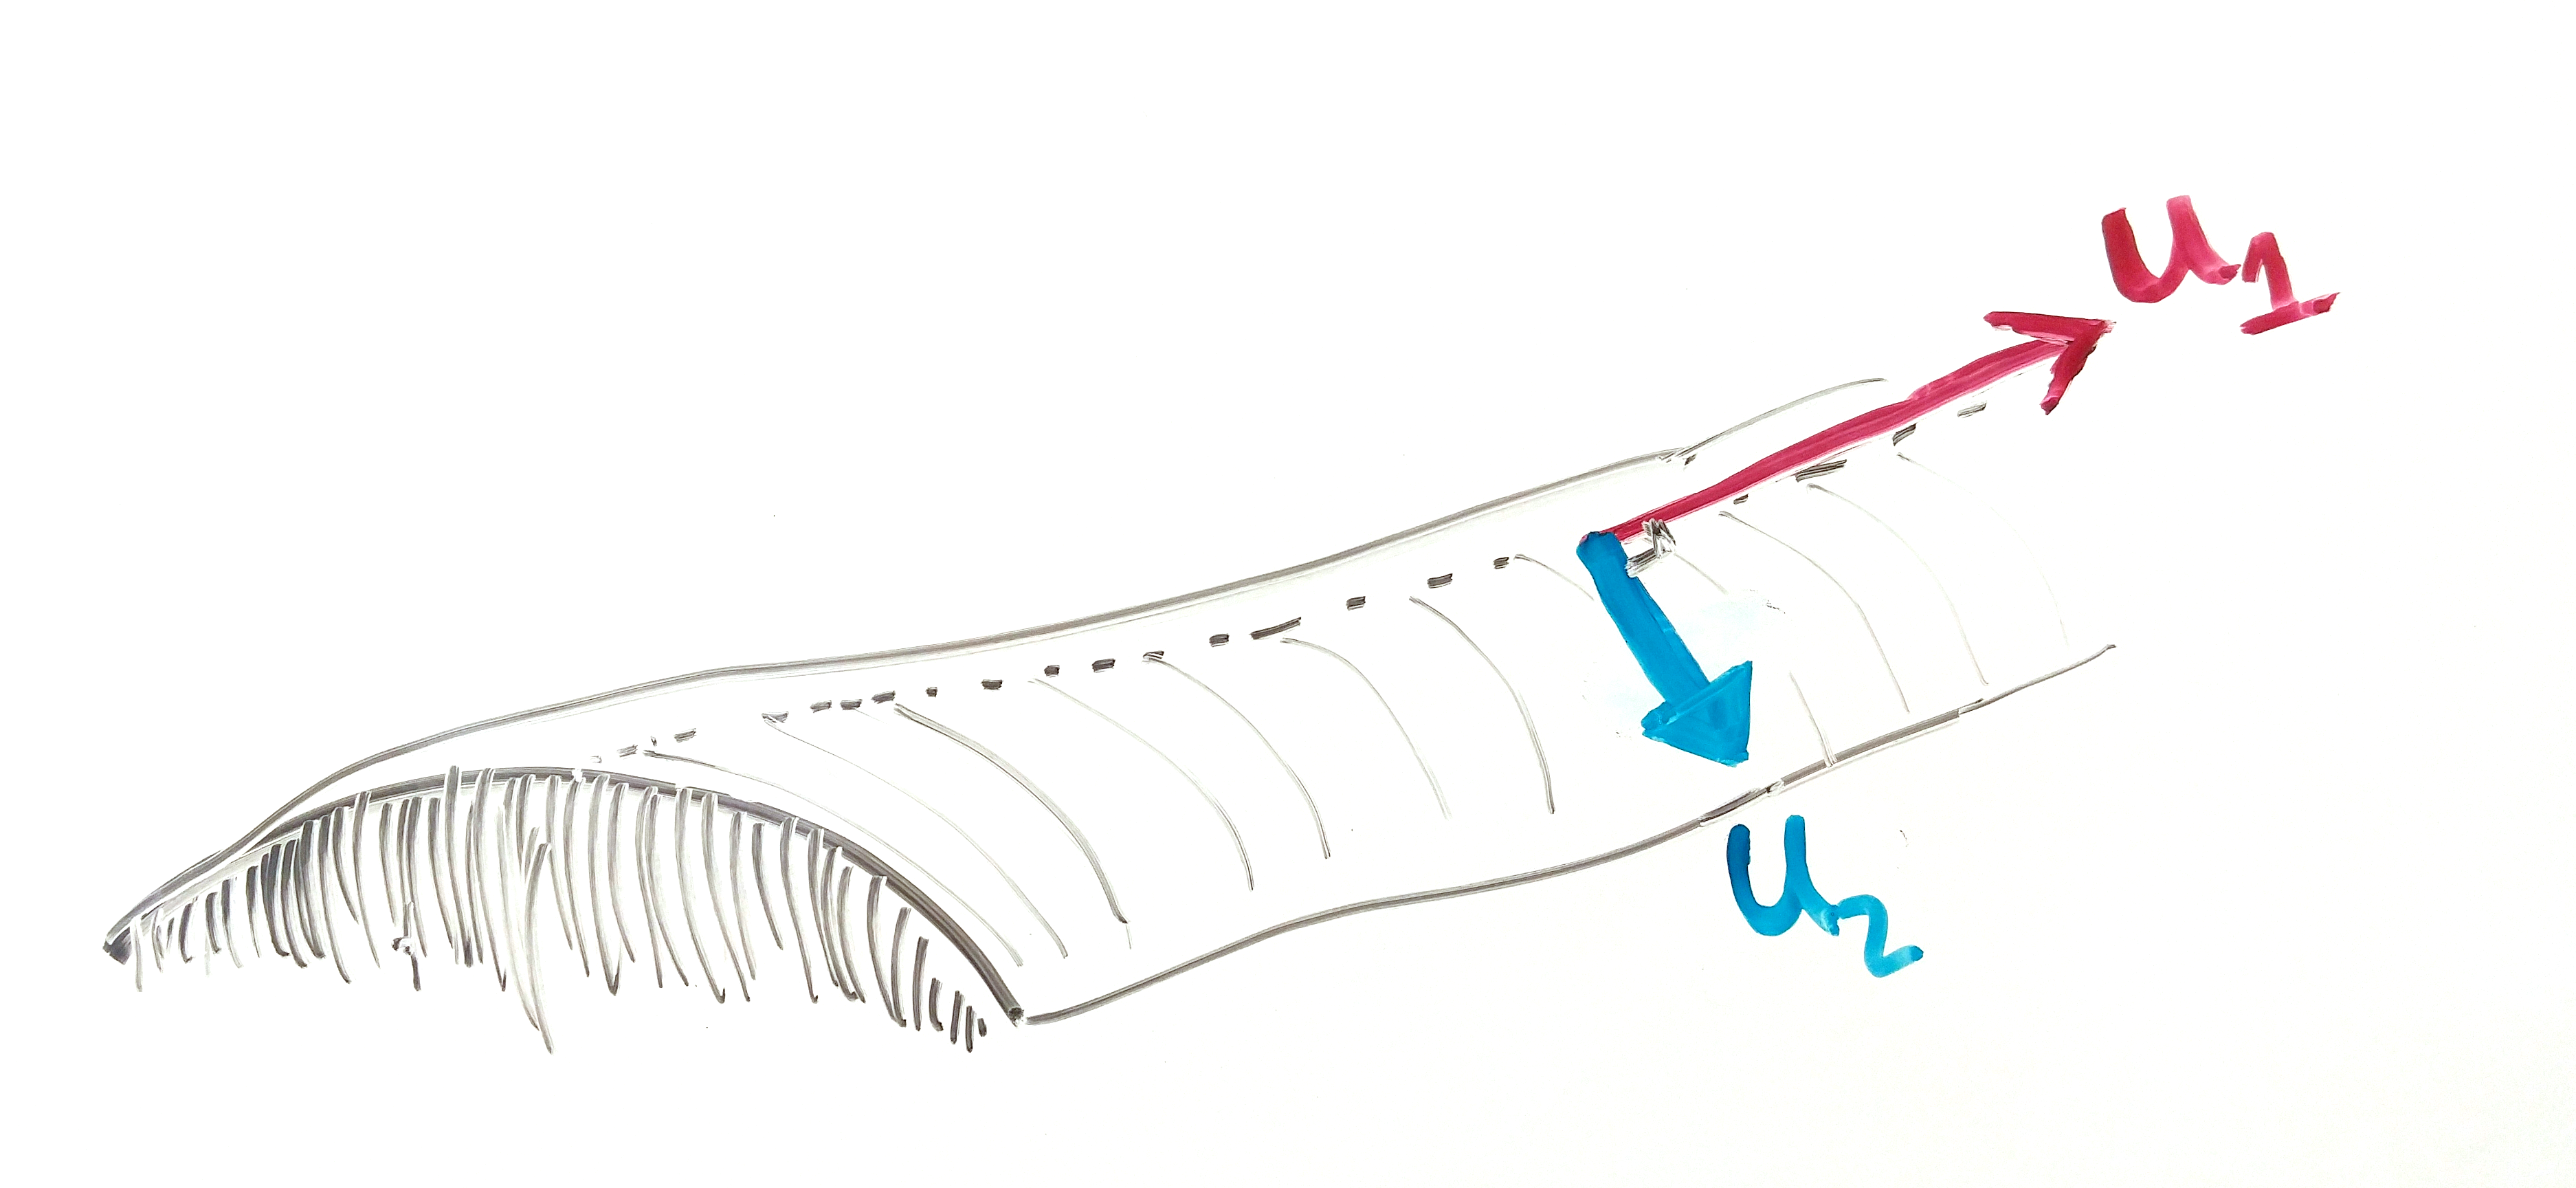
\includegraphics[width=0.8\linewidth]{expo_principal_curvatures}
    		\caption{The principal eigenvectors at a ridge like structure} 
    	 \label{fig:expo-principal-curvatures}
    \end{figure}
    
    In \cref{fig:expo-principal-curvatures}, this situation is demonstrated. Here, $u_1, u_2$ form the orthogonal set of Hessian eigenvectors with corresponding eigenvalues $\lambda_1$ and $\lambda_2$. At such a ridgelike structure, we could predict the largest change in curvature to be straight down the ridge (in the direction of $u_2$), and the direction of least curvature to be directly along the ridge (in the direction  of $u_1$). $\lambda_1 \approx 0$ and $\lambda_2$ is large and negative  Note that the length of these vectors in this picture is not meant tor represent their magnitudes, as $u_2$ should have a much larger relative magnitude by design!
    
    Of course, if the the ridge is perfectly circular along its cross section (as was in \cref{sec:calculate-weinmap-of-a-ridge}, it is of course apparent that $\lambda_2$ would be the same value at any place along the ridge (not just at its crest \vcleanup{fix terminology}), and $\lambda_1$ would likewise be 0 at any such point.  One could also imagine a similar situation in which the dropoff from crest to bottom gets increasing steep. In such a case, $\lambda_2$ as a function of $x$ would in fact be largest nearest to the bottom. This thought experiment should dispel a na\"{i}ve misunderstanding of the power of a Frangi filter: a high anisotropy measure (and a large structureness measure \vcleanup{define structureness first}) will not in general identify the crests of a ridge-like structure--it only will highlight that such a pixel is on a ridge-like structure at all. Thus, the anisotropy measure will not necessarily be at a maximum at the crest of the ridge, but instead, somewhere along it.
    
    Similiarly, the vessel we we wish to identify can not be reasonably expected to behave as perfectly as our toy example. There will likely be small aberrations in a ridgelike structure, such as small divots or depressions in an overall ridge-like structure. Of importance in our data set later ( \cref{sec:NCS-data-set}), there will be points where we seem to "lose" our ridgelike structure,
    but this is simply due to an error in the sample.
    
	Importantly, this formulation does not require $\lambda_1$ to be approximately zero, just that the curvature in the downward direction is much more significant.
    
    Also the crest could be really flat (``hangar shaped''), in which case both are around zero. At the crest of the ridge, we would actually expect both $u_1$ and $u_2$ to be around 0, whereas a point somewhere between the crest and the ``foot'' of the ridge to contain the maximum $u_2$.
    
    We will fix some of these issues by casting this as a multiscale problem in \cref{sec:frangi-multiscale}.
    
    Two other ideas that could fix some other discrepancies mentioned above is to identify these ridges on their own, or also where the 'feet are'. We will discuss these ideas in \cref{sec:future-research-directions}.
    
    \subsection{Structureness measure} \label{sec:frangi-structureness}
    
    There is another concern with using the pure ratio $S:= \abs{\lambda_1 / \lambda_2}$ as an identifying feature of ridgelike structures apart from the ones listed above. We could still have $\abs{\lambda_2} \gg \abs{\lambda_1}$ in a relative sense, but still have $\lambda_2 \approx 0$. As a rather extreme example, we should certainly wish to differentiate a point on the surface where $\lambda_2 \approx 10^{-5} $ and $\lambda_1 \approx 10^{-10}$ from another point where $\lambda_2 \approx 10000$ and $\lambda_2 = 0.1$.
    
    A natural fix to differentiate these points is to introduce a ``structureness'' measure to insure that there is in fact significant curvilinear activity at the point in question. Frangi used $S:= \sqrt{(\lambda_1)^2 + (\lambda_2)^2}$, which is in fact the Frobenius norm of the Hessian matrix. Thus the Frangi filter should also prefer areas of
    great curvilinear content in the image first of all.
    
    
    \subsection{The Frangi vesselness measure}
    
    Our goal then is to attach a numerical measure to each pixel in the image (at a particular scale $\sigma$) that is large when the anisotropy measure $A$ and the structureness measure $S$ is sufficiently large.
    
    The form Frangi arrived at in \cref{eq:frangi-vesselness-measure} in which a factor of $\exp\{...\}$ and $(1 - \exp\{...\})$ are multiplied together are simply to ensure that the final vesselness measure $V$ is largest when $A$ is small and $S$ is large enough, with rapid decay in other situations.
    
 Frangi further strengthened the filter by adding an additional case to in \cref{eq:frangi-vesselness-measure}, ensuring that $\lambda_2$ is not positive. If we are indeed at a curvilinear ridge, we need the second derivative of the surface in the maximal direction to be negative, which hasn't been accounted for as yet in our formulation of $A$ and $S$ -- we wish (for our purposes) to only identify when we are finding crests. $A$ will still be small and $S$ will still be large however if we identify a ``trough''.
 
 The only perceivable difference is that the maximum normal curvature will be positive--we are at a local minimum in the direction of $u_2$. In situations where we wish to only identify ridges (as is the case here) we simply exclude any points where there is not a negative curvature in the maximal direction. Conversely, we could only seek to find valley, or local minima, as thus require $\lambda_2 > 0$, and set the vesselness measure to zero when $\lambda_2 < 0$.
    
    \subsection{The Frangi vesselness filter: Choosing parameters $\beta$ and $c$}
    
    The parameters $\beta$ and $c$ are meant to scale so that the peaks of the anisotropy factor $\exp\{\frac{-A^2}{2\beta^2}\}$ and the structureness factor $(1-\exp\{\frac{-S^2}{2c^2}\})$ coincide enough to be statistically significant at highly curvilinear structures, but rapidly decay in areas not associated with curvilinear content. What values of these parameters are appropriate is ultimately dependent on the context of the problem.
    
    Frangi suggested for $c$ that half of (the Frobenius norm of the) Hessian matrix is appropriate, simply because the minimum value of $S$ is zero, and its maximum value is exactly the max Frobenius norm. With this in mind we would like to introduce the scaling factor
    $\gamma$, so that $ c = \gamma S_{\max}$. This creates a minor annoyance though: although the anisotropy factor can certainly attain a value of 1, if $c$ is to take this ``appropriate'' value, the maximum value of the structureness factor is somewhat smaller than 1. In fact,
    \begin{equation}
    \begin{aligned}
    \max\{V_\sigma\} &\le \max\left(
                                    \exp\left\{\frac{-A^2}{2\beta^2}\right\}
                            \right)
                        \max\left(
                            \left(1 - \exp\left\{\frac{-S^2}{2(\gamma S_{\max})^2}\right\}\right)
                            \right) \\
                    &\le \max\left\{
                    \left(1 - \exp\left\{\frac{-S^2}{2(\gamma S_{\max})^2}\right\}\right)
                    \right\} \\
                    &= 
                    \left(1 - \exp\left\{\frac{-(S_{\max})^2}{2(\gamma S_{\max})^2}\right\}
                    \right)
                    = \left(1 - \exp\left\{\frac{-1}{2\gamma^2}\right\}
                    \right)
    \end{aligned}
    \end{equation}
    
    Thus, when $\gamma$ takes the suggested value of $\gamma = 1/2$, the above calculation suggests that
    the maximum theoretical value that the Frangi filter could attain is
    $ \max \{ V_\sigma \} \le 1 - \exp\left\{ -1 \right\} \approx .8647$.
    This certainly explains why 
    \begin{equation} \label{eq:frangi-vesselness-measure-v1}
    V_\sigma(x_0,y_0) = \begin{cases}
    0 & \text{if} \quad \lambda_2 > 0 \\
    \exp\left\{\frac{-A^2}{2\beta^2}\right\}
    \left(1 - \exp\left\{\frac{-S^2}{2(\gamma S_{\max})^2}\right\}\right) & \text{otherwise}
    \end{cases} \end{equation}
    where, as before, 
    \begin{equation} \label{frangi-def-anisotropy-structureness-v1}
    A := \abs{\lambda_1 / \lambda_2}
    \quad \textrm{and} \quad 
    S := \sqrt{\lambda_1^2 + \lambda_2^2}
    \end{equation}
    
    For $\beta$ Frangi chose an innocuous intermediate point, $\beta=1/2$ (and thus $2\beta^2 = 1/2$).
    As we will show later, choosing the structureness parameter $\gamma$ is rather important for the context especially if the background (non-ridgelike structure) is significant and noisy. $\beta$ should be strengthened/relaxed depending on how ``flat'' the ridgelike structure is. If there is a lot of gain then $\beta$ should be smaller. If this is not the case, a stronger filter can be created by requiring $A$ to be much smaller.
    
    Considering as the anisotropy measure $(\lambda_1 / \lambda_2) \in [0,1]$ (simply since $\abs{\lambda_1} \ge \abs{\lambda_2}$), we can actually visualize how much the 
    anisotropy factor varies depending on our choice of $\beta$, as seen in \cref{fig:anisotropy-parameter-demo}.
    
    \begin{figure}
      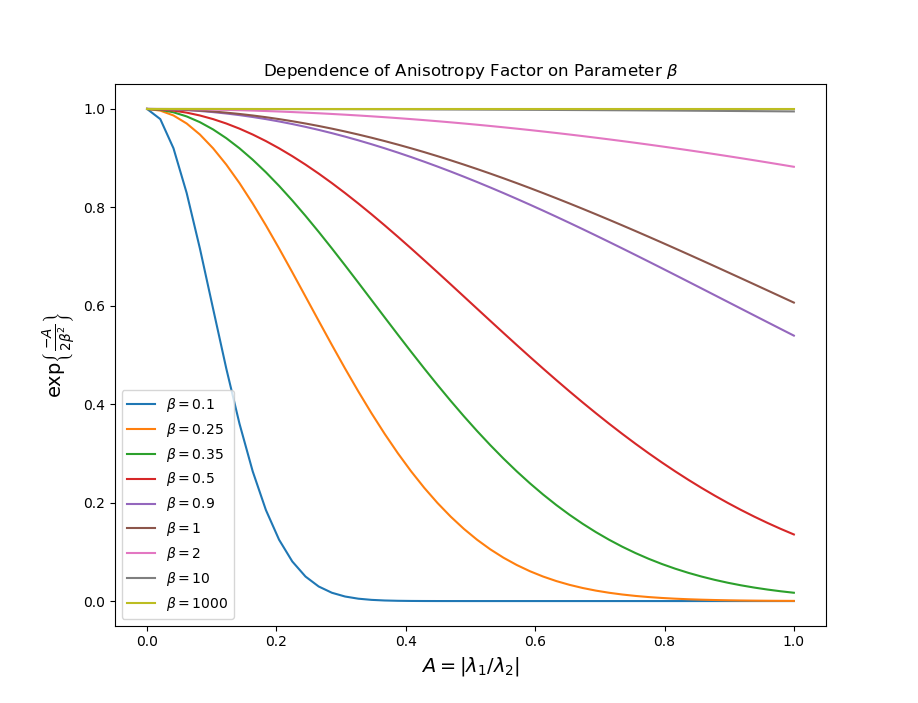
\includegraphics[width=\linewidth]{anisotropy_parameter_demo}
      \caption{Dependence of the Anisotropy Factor on its Parameter}
      \label{fig:anisotropy-parameter-demo}
    \end{figure}

We make a similar presentation of the dependence of the structureness kernel on its parameter $\gamma$, as you can see in
\cref{fig:structureness-parameter-demo}
    \begin{figure}
    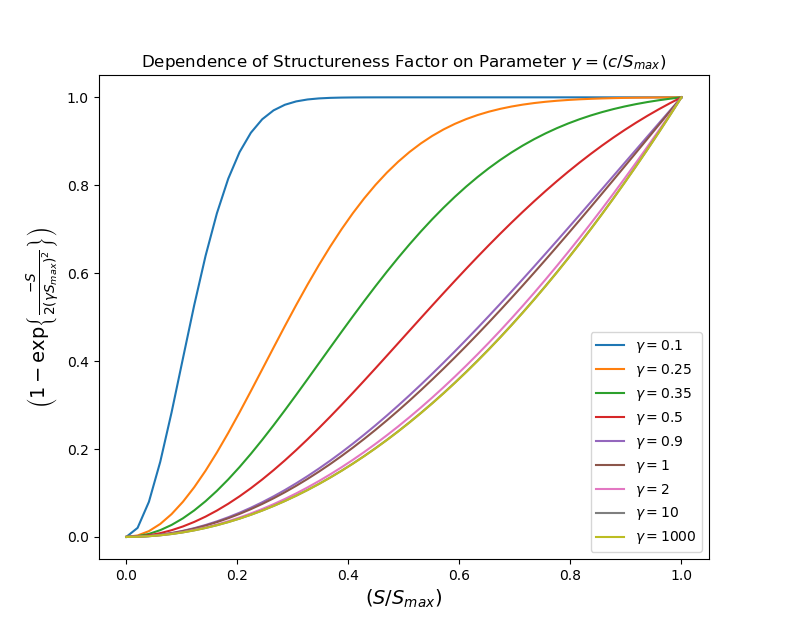
\includegraphics[width=\linewidth]{structureness_parameter_demo}
    \caption{Dependence of the Structureness Factor on its Parameter}
    \label{fig:structureness-parameter-demo}
  \end{figure}





	We now take a quick tangent from our description of the Frangi filter to develop and justify our ``multiscale'' approach.
	
        
    \section{Linear Scale Space Theory} \label{sec:scale-space-theory}
    
    
    There is obviously a major disconnect in the ideas presented above. 
    Although the ideas presented above require differentiation of continuous
    surfaces, our image is in fact a discrete pixel. That is, our previous discussions have been in terms of an image as the continuous surface in \cref{def:image_as_surface},
    rather than the more realistic discrete pixel matrix as in \cref{def:image_as_pixel_matrix}.
    The present section seeks to address this disconnect.
    In particular, we seek to mitigate the bias of our limited sampling
    of the ``true'' 3D surface. Our main goal is to counter against some of the bias of our particular sampling. In particular, we wish to not over-represent structures that
    are clear at our resolution without giving appropriate weight to larger structures as well.
    Koenderink \cite{Koenderink} argued that "any image can be embedded in a one-parameter family of derived images (with resolution as the parameter) in essentially only one unique way" given a few of the so-called scale space axioms. He (and others) showed that a small set of intuitive axioms imply require that any such family of images must satisfy the heat equation
    
    \begin{equation} \label{eq:heat-eq-for-family}
    \Delta K(x,y,\sigma) = K_\sigma (x,y,\sigma) 
    \;\text{for}\; \sigma \ge 0
    \;\text{such that}\; K(x,y, 0) = u_0(x,y).
    \end{equation}
    
    where $K: \R^3 \to \R $ and  $u_0: \R^2 \to \R: $ is the original image (viewed as a continuous surface) and $\sigma$ is a resolution parameter.
    Much work has been done to formalize this approach \cite{GSST-book}. There is a long list of desired properties--we will to try to identify a minimal subset of axioms and show that other desired properties follow.
    
	  
    
    \subsection{Axioms}
	 To make matters manageable, we require the one-parameter family of scaled images to be generated by an operation on the original image:
	 
	\[
		\left\{\ K(x,y;\sigma) = T_\sigma u_0
		\ \lvert \ 
		\sigma \ge 0
		\; ,\; K(x,y,;0) = u_0
		\ \right\} 
	\]
    
	The following axioms are then requirements on what sort
	of operation $T_\sigma$ should be.
		
    \begin{axiom}[Linear-shift and Rotational Invariance]
    	\label{axiom:linear-shift-and-rotation}
    Linear-shift (or translation) invariance means that no position in the original signal is favored.  This is intuitive, as our operation should apply to any image fairly, regardless of where content is found in the image. Similarly, there should be not be favoritism toward any particular orientation of content within the image.
\end{axiom}
    
    \begin{axiom}[Continuity of Scale Parameter]
    	\label{axiom:continuity} There is no reason for the scale parameter to be discrete; we may alter the resolution with whatever
    precision we desire. That is, we take the resolution
    parameter $\sigma$ to be a nonzero real number
    (as opposed to an integer). Moreover, we require that the operator behaves continuously with respect to the scale parameter.
        \end{axiom}
    What happens as $\sigma \downarrow 0$ is not immediately clear though. 	An argument from functional analysis (see \cite{hille1957functional}) implies that there is a so-called ``infinitesimal generator'' $A$
	which is a limit case of our desired operator $T$; that is
	\begin{equation} \label{eq:infinitesimal-generator}
	A u_0 = \lim_{\sigma \downarrow 0} \frac{T_\sigma u_0 - u_0}{\sigma}
	\end{equation}
	 
	 and moreover that there is a resultant differential equation
	 concerning the derivative of the family and $A$:
	 
	 \begin{equation}
	 \partial_{\sigma} K(x,y;\sigma)
	 = \lim_{\sigma \downarrow 0}
	 \frac{K(\cdot;\sigma+h) - K(\cdot; \sigma)}{h}
	 = A(T_\sigma u) = A(K(\cdot,\sigma))
	 \end{equation}
	 
	 We shall return to this idea later and more concretely describe $A$ once we actually characterize the generating 
	 operator $T_\sigma$.
    
    \begin{axiom}[Semigroup property] \label{axiom:semigroup}
    The semigroup property is simply that transforming
    the original image by some resolution $\sigma$ should
    have the same overall effect of two successive
    transformations $\sigma_1$ and $\sigma_2$, i.e.
    
    \begin{equation}	
	    T_{\sigma} u = T_{\sigma_1 + \sigma_2} u
    \end{equation}
    \end{axiom}
%     \subsubsection{Linearity of generator}
%        ``Linearity implies that all-scale space properties valid for the original signal will transfer to its derivatives. Hence, there is no commitment to certain aspects of image structure, such as the zero-order representation, or its first- or second-order derivatives.''
   

   \begin{axiom}[Causality Conditon] \label{axiom:causality}
    The following requirement has great implication, and is also
    very successful in encoding our intuitive sense
    of ``resolution''. The causality condition is the one
    that, as resolution decreases, no finer detail is
    introduced into the image. That is, as the scale
    increases, there will be no creation of local extrema
    that did not exist at a smaller scale.
    \end{axiom}
    In other words, if 
    $K(x_0,y_0 ; \sigma_0)$ is a local maximum (at the point $(x_0, y_0)$, at this fixed $\sigma_0$)
    i.e. 
    then an increase in scale can only weaken this peak, i.e.
    \begin{equation}
    \left\{\begin{aligned}
    \nabla K(x_0,y_0; \sigma_0) &= 0 \\
    \Delta K(x_0,y_0;\sigma_0) &< 0
    \end{aligned}\right.
	\quad \implies \quad
	K(x_0,y_0;\sigma_1) \le K(x_0,y_0;\sigma_0)
	\; \forall\; \sigma_1 \ge \sigma_0
    \end{equation}
    
    Similarly, if $K(x_0,y_0;\sigma_0)$ is a local minimum (with respect to space), then an increase in scale cannot make such a valley more profound, i.e.
   \begin{equation}
   \left\{\begin{aligned}
   \nabla K(x_0,y_0; \sigma_0) &= 0 \\
	\Delta K(x_0,y_0;\sigma_0) &> 0
	\end{aligned}\right.
	\quad \implies \quad
	K(x_0,y_0;\sigma_1) \ge K(x_0,y_0;\sigma_0)
	\; \forall\; \sigma_1 \ge \sigma_0
	\end{equation}
    
    This implies that no image feature is sharpened by an decrease and resolution--the only result is a monotonic blurring of the image as scale parameter $\sigma$ tends to infinity.


    \subsection{Uniqueness of the Gaussian Kernel}
    
    The above requirements are actually sufficient in proving not only that the operator $T_\sigma$ is a convolution, but that the heat equation described in \cref{eq:heat-eq-for-family} must hold. This has been shown in various ways, both by Koenderink \cite{Koenderink}, Babaud \cite{babaud}, as well as Lindeberg in \cite{GSST-book}. In fact, it is shown that the Gaussian is the unique convolution kernel that works.    
    
   To this, show that:
    \begin{itemize}
    \item a kernel satisfying the above axioms must satisfy the heat equation
  	\item the gaussian kernel satisfies that.
    \item gaussian kernel is the only kernel that works.
    \end{itemize}
    
    That is,
    \begin{equation}
   K(x,y;\sigma) = T_{\sigma} u_0 = G_\sigma \star u_0
   	\quad \textrm{where}\quad
   	G_\sigma := \frac{1}{2\pi \sigma^2} e^{\left(-\abs{x}^2 / (2\sigma^2)\right)}
    \end{equation}
    
	We can show that this solution solves the heat equation.
	Given $u_0$ as a continuous image (unscaled),
	we construct PDE with this as a boundary condition.
    
    \begin{equation}
    u: \R^2 \supset \Omega \to \R \; \textrm{with} \; u(\bm{x},t) : \;
    \begin{cases}
    \frac{\partial u}{\partial t} (\bm{x}, t) = \Delta u(\bm{x},t) & ,\; t \ge 0 \\
    u(\bm{x},0) = u_0(\bm{x}) 
    \end{cases}
    \end{equation}
    
    We show that
    \begin{equation}
    u(\bm{x},t) = \left(G_{\sqrt{2t}} \star u_0 \right)(\bm{x})
    \end{equation}
    solves (the above tagged equation), where
    \[
    s
    \]
    First, we need a quick lemma regarding differentiation a continuous convolution.
    \begin{lemma} \label{dconvolution}
    	Derivative of a convolution is the way that it is (obviously rewrite this).
    \end{lemma}
    \begin{proof}
    	For a single variable,
    	\begin{align}
    	\frac{\partial}{\partial \alpha} \left[ f(\alpha) \star g(\alpha) \right]
    	&= \frac{\partial}{\partial \alpha} \left[ 
    	\int f(t) g(\alpha - t) dt \right] \\
    	&=  \int f(t) \frac{\partial}{\partial \alpha}\left[ g(\alpha - t)  \right] dt \\
    	&=  \int f(t) \left(\frac{\partial g}{\partial \alpha}\right) g(\alpha - t) dt \\
    	&=  f(\alpha) \star g'(\alpha)
    	\end{align}
    	By symmetry of convolution we can also conclude 
    	\[\frac{\partial}{\partial \alpha} \left[ f(\alpha) \star g(\alpha) \right]
    	= f'(\alpha) \star g(\alpha)
    	\]
    	
    	If $f$ and $g$ are twice differentiable, we can compound this result to show a similar statement holds for second derivatives, and then, given the additivity of convolution,
    	we may conclude
    	\begin{equation}
    	\Delta \left(f \star g \right) = \Delta(f) \star g = f \star \Delta(g) 
    	\end{equation} 
    \end{proof}
    \begin{theorem}
    	$u(\bm{x},t) = \left(G_{\sqrt{2t}} \star u_0 \right)(\bm{x})$ solves the heat equation.
    \end{theorem}
    \begin{proof}
    	We focus on the particular kernel
    	\[
    	G_{\sqrt{2t}} = \frac{1}{4\pi t} e^{\left(-\abs{x}^2 / (4t)\right)}
    	\]
    	
    	
    	Then
    	\begin{align}
    	\frac{\partial u}{\partial t} (\bm{x}, t)
    	&= \frac{\partial}{\partial t} \left(G_{\sqrt{2t}}(\bm{x},t) \star u_0(\bm{x})\right)  \\
    	&= \frac{\partial}{\partial t} \left(G_{\sqrt{2t}}(\bm{x},t)\right) \star u_0(\bm{x})  \\
    	&= \frac{\partial}{\partial t} \left(
    	\frac{1}{4\pi t} e^{\left(-\abs{x}^2 / (4t)\right)} \right) \star u_0(\bm{x}) \\
    	&= \left[
    	-\frac{1}{4\pi t^2} e^{\left(-\abs{x}^2 / (4t)\right)}
    	+ \frac{1}{4\pi t}\left(\frac{-\abs{x}^2}{4t^2}\right) e^{-\abs{x}^2 / (4t)}
    	\right] \star u_0(\bm{x}) \\
    	&= -\frac{1}{4t^2} \left( e^{\left(-\abs{x}^2 / (4t)\right)} 
    	+ \abs{\bm{x}}^2 G_{\sqrt{2t}}(\bm{x},t)
    	\right) \star u_0(\bm{x})
    	\end{align}
    	and from the previous lemma,
    	\[
    	\Delta u(\bm{x}, t) = \Delta\left( G_{\sqrt{2t}} \star u_0(\bm{x})\right)
    	= \Delta\left( G_{\sqrt{2t}} \right)\star u_0(\bm{x})
    	\]
    	
    	We explicitly calculate the Laplacian of $G_{\sigma}(x,y) = A \exp(-\frac{x^2 + y^2}{2\sigma^2})$ as follows:
    	
    	\begin{align*}
    	\frac{\partial}{\partial x} G_{\sigma}(x,y)
    	&= A \left( \frac{-2x}{2\sigma^2}\right) \exp\left(-\frac{x^2 + y^2}{2\sigma^2}\right) \\
    	\implies \frac{\partial^2}{\partial^2 x} G_{\sigma}(x,y)
    	&= A \cdot \frac{\partial}{\partial x}
    	\left[ - \frac{x}{\sigma^2} \exp\left(-\frac{x^2 + y^2}{2\sigma^2}\right) \right] \\
    	&= A \left[ - \frac{1}{\sigma^2} \exp\left(-\frac{x^2 + y^2}{2\sigma^2}\right) 
    	+ \frac{x}{\sigma^2} \cdot \frac{2x}{2\sigma^2} \exp\left(-\frac{x^2 + y^2}{2\sigma^2}\right) \right] \\
    	&= A \exp\left(-\frac{x^2 + y^2}{2\sigma^2}\right)
    	\left[ - \frac{1}{\sigma^2} + \frac{x^2}{\sigma^4} \right] \\
    	&= \frac{1}{\sigma^2} G_\sigma(x,y)  \left[ \frac{x^2}{\sigma^2} - 1\right]
    	\end{align*}
    	
    	By symmetry of argument we also may conclude
    	\[
    	\frac{\partial^2}{\partial y^2} G_{\sigma}(x,y) = \frac{1}{\sigma^2} G_\sigma(x,y)  \left[ \frac{y^2}{\sigma^2} - 1\right]
    	\]
    	
    	and so
    	
    	\begin{equation}
    	\Delta G_\sigma(x,y) =
    	\frac{\partial^2}{\partial x^2} \left(G_{\sigma}\right)
    	+ \frac{\partial^2}{\partial y^2} \left(G_{\sigma}\right)
    	= \frac{1}{\sigma^2} G_\sigma(x,y) \left[ \frac{x^2 + y^2}{\sigma^2} - 2\right] 
    	\end{equation}
    	Then, given \cref{dconvolution}, we conclude
    	\begin{equation}
    	\Delta \left[ G_\sigma(x,y) \star u_0(x,y) \right] 
    	= \left(\frac{1}{\sigma^2} G_\sigma(x,y) \left[ \frac{x^2 + y^2}{\sigma^2} - 2\right]\right) \star u_0(x,y)
    	\end{equation}
    	
    	For particular choices of $\sigma(t) = \sqrt{2t}$ and $A = \frac{1}{4\pi t}$,
    	we see 
    	\begin{align}
    	\Delta \left[ G_{\sqrt{2t}}(x,y) \star u_0(x,y) \right] 
    	&= \left(\frac{1}{2t} G_{\sqrt{2t}}(x,y) \left[ \frac{x^2 + y^2}{2t} - 2\right]\right) \star u_0(x,y) \\
    	&= \left(G_{\sqrt{2t}}(x,y) \left[ \frac{x^2 + y^2}{4t^2} - \frac{1}{t}\right]\right) \star u_0(x,y)
    	\end{align}
    	We then calculate the time derivative,
    	using our particular choice of $\sigma(t) = \sqrt{2t}$ and $A = \frac{1}{4\pi t}$ as:
    	
    	\begin{align}
    	\frac{\partial}{\partial t} \left[ G_{\sigma(t)}(x,y) \star u_0(x,y) \right]
    	&= \frac{\partial}{\partial t} \left[ G_{\sigma(t)}(x,y) \right] \star u_0(x,y) \\
    	&= \frac{\partial}{\partial t} \left[ G_{\sqrt{2t}}(x,y)\right] \star u_0(x,y) \\
    	&= \frac{\partial}{\partial t} \left[
    	\frac{1}{4\pi t} \exp\left(-\frac{x^2 + y^2}{4t}\right) \right] \star u_0(x,y) \\
    	&= \left[ -\frac{1}{4\pi t^2} \exp\left(-\frac{x^2 + y^2}{4t}\right) + 
    	\frac{1}{4\pi t}\left( \frac{x^2 + y^2}{4t^2} \exp\left(-\frac{x^2 + y^2}{4t}\right)\right)
    	\right] \star u_0(x,y) \\
    	&= \left(G_{\sqrt{2t}}(x,y) \left[ \frac{x^2 + y^2}{4t^2} -\frac{1}{t}\right]\right) \star u_0(x,y)
    	\end{align}
    	
    	Combining these results, we find that
    	\begin{equation}
    	\frac{\partial}{\partial t} \left[ G_{\sqrt{2t}} \star u_0 \right]
    	= \Delta \left[ G_{\sqrt{2t}} \star u_0 \right] 
    	\end{equation}
    	
    	as desired. \end{proof}
    
    
    
    \subsection{Scale Spaces over Discrete Structures} \label{subsec:discrete-scale-space}
    
    The above developments from scale space axioms have (since their first appearance)
    been recast in terms of discrete structures (rather than continuous surfaces) as in \cite{lindeberg-discrete}. However, we've chosen to present the above in their original continuous surface for clarity of argument. The discrete case is not much different--
    we still have the same axioms, and it can be shown that the family of scaled images
    must simply satisfy a discrete version of the 
    However, viewing our actual image
    \cref{def:image_as_pixel_matrix} as a sample of a continuous
    surface \cref{def:image_as_surface},
    we might na{\"i}vely expect our convolution by the Gaussian to ``commute'' with our supposed sampling of the continuous signal,
    or even that we could simply convolve our discrete signal with a discretely sampled Gaussian kernel. The latter in fact, seems to be an often implemented interpretation of scale space theory.
    
    To be clear, the ``sampled'' 1D Gaussian Kernel we have in mind might be given by:
   
    \begin{defn}[Sampled Gaussian Kernel and Generated Family]
    	\[
    	g(n ; \sigma) = \frac{1}{2\pi \sigma} e^{-n^2 / 2\sigma} \;,\quad -\infty < n < \infty
    	\]
    	\end{defn}
    and the  resulting (1D) convolution would be given by
    \[
	    K(x,\sigma) = \sum_{n=-\infty}^{\infty} g(n;\sigma) f(x-n)
	    \quad \textrm{for} \quad x \in \Z, \; \sigma > 0
    \]
    The reality of the matter is that a discretely sampled Gaussian is not an appropriate kernel for creating discrete scale space. In \cite{lindeberg-discrete} and in particular
    \cite{lindeberg1988-discreteconstruction}, Lindeberg demonstrated that the sampled Gaussian kernel violates not only semigroup property (\cref{axiom:semigroup}), but--much less forgivably--the causality property (\cref{axiom:semigroup}). There is absolutely no guarantee that convolution with a sampled Gaussian kernel will not create ``spurious'' structures as resolution increases.
    
    
    Fortunately, Lindeberg was immediately able to remedy this by providing a discrete analogue of the Gaussian kernel, which does satisfy \cref{axiom:causality} and \cref{axiom:semigroup}:
    
    \begin{defn}[Discrete Gaussian Kernel]
    	The discrete Gaussian kernel, which can be shown to be a suitable generator
    	for scale space, is given by
    	\begin{equation}
    	T(n;\sigma) = e^{-\alpha \sigma} I_n(\alpha \sigma) ,\quad\,
    	 I_n(\sigma) = I_{-n}(\sigma) = (-1)^n J_n(i\sigma) 
    	 \quad n \ge 0 , \sigma,\alpha > 0
    	 \end{equation}
    \end{defn}
    where $I_n$ are the modified Bessel functions of integer order based on the
    ordinary Bessel functions $J_n$, i.e.
    \[
    I_n(x) = \sum_{m=0}^{\infty} \frac{1}{m! (m+n)!}
	    	\left(\frac{x}{2}\right)^{2m+n} \;,\quad n \ge 0
    \]
    where we have taken the liberty of simplifying the typical definition \cite{abramowitz-stegun} (which involves the gamma function), since we only desire
    Bessel functions of integer order. The parameter $\alpha$ above is simply an
    optional scaling parameter which is simply set to $1$ hereforth.
    
    The derived family of 1D signals is then given by
\begin{equation} \label{eq:derived-family-from-discrete}
        K(x,\sigma) = \sum_{n=-\infty}^{\infty} T(n;t) f(x-n)
        \quad \textrm{for} \quad x \in \Z, \; t > 0
        \end{equation}
    
    The compatibility of scale space theory and derivatives on discrete structures and     extension to two dimensions was also demonstrated by Lindeberg in \cite{lindeberg-discrete-derivative} and \cite{lindeberg1998feature}. In particular, we may take derivatives of the convolutions of our discrete images
    using, say, a central difference.
    Lastly, the 2D version of the family given in \cref{eq:derived-family-from-discrete} can be obtained by independent convolution of its dimensions (i.e. it is separable). We will make these
    ideas explicit in \cref{ch:implementations} and the Appendix.
    
    With the ideas of scale established, we may return to our discussion of the Frangi filter.
    
    \section{The Frangi Filter: A multiscale approach} \label{sec:frangi-multiscale}
    
    Our ideas of scale developed in the previous section imply that, if the ridgelike structures we wish to detect are more prominent at different scales, then a multiscale approach is the natural one. Considering our
    developments in \cref{sec:frangi}, we wish to probe at multiple scales
    regions that would receive a high vesselness score at any range,
    and consider them all together. Frangi \cite{frangi-paper} approached this problem by simply aggregating vesselness measure over all scales:
    
    \begin{equation} \label{frangi-vesselness-max}
    V(x_0, y_0) = \underset{\sigma \in \Sigma}{\max}\;  V_\sigma(x_0, y_0)
    \end{equation}
    
    where $\Sigma := \left\{ \sigma_0, \sigma_1 , \cdots, \sigma_N \right\}$ is
    a range of parameters at which to probe. These should be chosen to be representative enough of all scales where meaningful content is expected to be found.
    
    % move to Chapter 3.
    \subsection{Thresholding}
    
    After this procedure, we are left with a matrix with as many samples/pixels as the original image, all with a vesselness measure between $0$ and $1$ for each pixel in the image:
    
    \begin{equation} \label{eq:frangi-max-matrix}
    \mathsf{V}_\Sigma := \left[ V(x, y)\right]_{\substack{0\le x<M \\ 0\le y<N}}
    \end{equation}
    
    Notably, Frangi \cite{frangi-paper} refrained from explicitly interpreting the probablility assigned by \cref{frangi-vesselness-max}; that is--whether a particular point $(x,y)$ in the image definitely a vessel or not. Instead, he cautioned that the result should not be used as a segmentation method alone, and that the size
    of the vasculature cannot be determined rigorously from the filter alone.
    
    However, for the purposes of obtaining an intermediate result, we wish to be final about the whole matter and ultimately say whether or not a pixel does in fact corresponds to a curvilinear structure. A straightforward enough approach is to simply threshold at some fixed value. The resulting matrix can be given in terms of either \cref{frangi-vesselness-max} or \cref{eq:frangi-max-matrix}
    \vcleanup{fix notation in all of this}
    \begin{equation}
    V_{\Sigma,\alpha}(x,y) = \begin{cases}
    1 & \textrm{if}\quad V(x,y) \; \ge\;  \alpha \\
    0 & \textrm{else}
    \end{cases}  \quad , \quad \alpha > 0
	    \; \textrm{for } \; \alpha \;\textrm{fixed}.
    \end{equation}
    
	We will discuss alternatives methods of aggregating results from our multiscale method, as well as optimal values for parameters and scales
	in \cref{ch:implementations}. As a final note, we admit that any future extensions of this work (as will be discussed in \cref{ch:conclusion}) should not hold too much stock in this thresholded result, and analyzing the 
	raw vesselness score \cref{eq:frangi-max-matrix}, or even
	the un-merged scale-wise scores, would be far more
	rewarding.    
	

All that remains to describe mathematically is how to actually calculate the derivatives of our images and deal with the ultimately discrete nature of our samples.    
 
 
\section{Calculating the 2D Hessian}

According to \cref{subsec:discrete-scale-space}, we may calculate derivatives of our structure by calculating a gradient on our convolved image. Our method of calculating the gradient of a matrix uses a second-order accurate central difference, as in \cite{fornberg-1988}. Specific implementation will be discussed in \cref{ch:implementations}.

We note in passing that we may take the derivative of the Gaussian kernel and then convolve it, and the effect will be the same as if we had taken the derivative subsequently \cite{DIPGW}. This could offer some computational speedup if we wish to run this procedure on many samples and fixed scale sizes, although we have implemented our scale spaces in the conventional way, as discussed in \cref{ch:implementations}.
%Given that we are taking a derivative of a convolution, we first show that these operations commute--that is, we may actually take the derivative of the convolution kernel OR the function itself, and then convolve, and the result should be equivalent to taking the derivative of
%convolving 

%Note the following 6 methods should all theoretically be equivalent:
%
%\begin{itemize}
%   	\item convolve discrete image with a gaussian kernel, then take derivatives (no FFT). This is the ``classical approach''
%   	\item Take derivatives of gaussian kernel, then convolve with the image/signal (again, no FFT)(due to \vcleanup{cite theorem})
%   	\item FFT image and FFT gaussian kernel then convolve in freq. space, then IFFT, then take derivatives in xy-space (my implementation)
%   	\item take derivatives of gaussian kernel, then FFT it,  FFT the image, then colvolve in frequency space, then  IFFT (slower due to size of large kernels)
%   	\item FFT image, then multiply by theoretical gaussian kernel in freq. space, then IFFT, then take derivatives in xy-space.
%   	\item FFT image, then multiply by theoretical gaussian kernel in freq space, then take derivatives in freq space, then IFFT.
%   	
%   	
%\end{itemize}


\section{Convolution Speedup via FFT}

In practice, the convolutions described above  are very slow for large scales ($\large \sigma$), as the size of the kernel is very large. Instead, we will perform a fast Fourier transform, which requires only $\mathscr{O}\left(N\cdot \log_2N\right)$ operations for a one dimension signal of length $N$, as compared to the $N^2$ operations required of a conventional discrete Fourier transform \cite{DIPGW}. We will briefly outline the theory of Fourier transforms.

\subsubsection{Fourier Transform of a continuous 1D signal}

\vcomment{start with 1D but then extend/rewrite}

A periodic signal (real valued function) $f(t)$ of period $T$ can \vcomment{justify?} be expanded in an infinite basis as follows:

\begin{equation}
f(t) = \sum_{-\infty}^{\infty} c_n e^{i\frac{2\pi n}{T}t} \;,\quad
	c_n = \frac{1}{T}\int_{-T/2}^{T/2} f(t) e^{-i\frac{2\pi n}{T}t} dt
	\end{equation}

The Fourier transform of a 1D continuous function is defined by
\begin{equation} \label{1D-CFT}
F(\mu) := \FT\{f(t)\} \;=\; \int_{-\infty}^{\infty} f(t) e^{i2\pi \mu } dt
\end{equation}

An inverse transform will then recover our original signal:
\begin{equation} \label{1D-ICFT}
f(t) = \FT^{-1}\left\{F(\mu)\right\} = \int_{-\infty}^{\infty} F(\mu) e^{i2\pi \mu t} dt
\end{equation}

Together, \cref{1D-CFT} and \cref{1D-ICFT} are referred to as the \textit{Fourier transform pair} of the signal $f(t)$. 

\subsubsection{Fourier Transform of a Discrete 1D signal}

We wish to develop the Fourier transform pair for a discrete signal., following \cite{DIPGW}. We frame the situation
as follows: A continuous function $f(t)$ is represented as the sampled function $\tilde{f}(t)$ by multiplying it by a sampling (or impulse) function, an infinite series of discrete impulses with equal spacing $\Delta T$:

\begin{equation} \label{1D-sampling-function}
s_{\Delta T}(t) := \sum_{n=-\infty}^{\infty} \delta[t - n\Delta T] \;,\quad
\delta[t] = \begin{cases} 1 \;,\; & t=0 \\ 0 \;,\;& t \ne 0 \end{cases}
\end{equation}

where $\delta[t]$ is the discrete unit impulse.

The discrete sample $f(t)$ is then constructed from $f(t)$ by
\begin{equation} \label{1D-discrete-sample}
\tilde{f}(t) = f(t) s_{\Delta T}(t)
\end{equation}

From this we can calculate $\tilde{F}(t)$.
Given the discrete signal $\tilde{f}$, we construct the transform
$\tilde{F}(\mu) = \FT\{\tilde{f}(t)\}$. by expanding $\tilde{f}$ in the same infinite basis as the continuous case.
\begin{equation} \label{1D-DFT-transform}
\tilde{F}(\mu) = \sum_{n=-\infty}^{\infty} f_n e^{-i 2\pi \mu n \Delta T} \;,\quad
f_n = \tilde{f}(n) = f(n\Delta T)
\end{equation}

The transform is a continuous function with period $1 / \Delta T$. 

%\begin{itemize}
%	\item \vtodo{find image processing papers that find hessian from FFT / who uses this?}
%	\item \vtodo{with above: downsides?}
%	\item \vtodo{side by side comparison in a toy example and/or a real problem?}
%\end{itemize}

\subsubsection{2D DFT Convolution Theorem}\vcomment{the following was adapted in a large part from DFT: an owner's manual. cite? DIP-DW just proves the continous version (in 1D) and then asserts that it works for discrete variables too.}

\vcleanup{get consistent notation--either have the discrete signals be notated as  $\tilde{f}(x,y)$ or $f[x,y]$ or instead comment that it's understood}
\begin{theorem}[2D DFT Convolution Theorem] 
	\vcomment{develop the 2-D DFT from Sec. 4.3 4.4 from DIP-GW (see p235).}
Given two discrete functions are sequences with the same length.
%\vcomment{If they're not actually the same length, DIP-GW suggests to make the final length at least $P = A+C-1$ and $Q = B+D-1$ in the case that the sizes are $A\times B$ and $C\times D$ for $f(x,y)$ and  $h(x,y)$ respectively. Not sure if that matters.}
$f(x,y)$ and $h(x,y)$ for integers $0 < x < M$ and $0 < y < N$, we can take the discrete fourier transform (DFT) of each:
\begin{align}
F(u,v) := \mathcal{D}\{f(x,y)\} &=
				\sum_{x=0}^{M-1} \sum_{y=0}^{N-1} f(x,y)
				e^{-2\pi i \left(\frac{ux}{M} + \frac{vy}{N}\right)} \\	
H(u,v) := \mathcal{D}\{h(x,y)\} &=
				\sum_{x=0}^{M-1} \sum_{y=0}^{N-1} h(x,y)
				e^{-2\pi i \left(\frac{ux}{M} + \frac{vy}{N}\right)}
\end{align}

and given the convolution of the two functions
\begin{equation}
\left(f \star h\right)(x,y) = \sum_{m=0}^{M-1} \sum_{n=0}^{N-1} f(m,n)h(x-m,y-n)
\end{equation}

then $\left(f \star h\right)(x,y)$ and $MN\cdot F(u,v)H(u,v)$ are transform pairs, i.e.
\begin{equation}
\left(f \star h\right)(x,y) = \mathcal{D}^{-1}\left\{MN\cdot F(u,v)H(u,v)\right\}
\end{equation}
\end{theorem}


The proof follows from the definition of convolution, substituting in the inverse-DFT of $f$ and $h$, and then rearrangement of finite sums.
\begin{proof}
\begin{align}
\left(f \star h\right)(x,y) &= \sum_{m=0}^{M-1} \sum_{n=0}^{N-1} f(m,n)h(x-m,y-n) \\
&= \sum_{m=0}^{M-1} \sum_{n=0}^{N-1}
\left(\sum_{p=0}^{M-1} \sum_{q=0}^{N-1} F(p,q)
	e^{2\pi i \left(\frac{mp}{M} + \frac{nq}{N}\right)}\right)
	\left(\sum_{u=0}^{M-1} \sum_{v=0}^{N-1} H(u,v)
	e^{2\pi i \left(\frac{u(x-m)}{M} + \frac{v(y-n)}{N}\right)} \right) \\
&= \left(\sum_{u=0}^{M-1} \sum_{v=0}^{N-1} H(u,v)
	e^{2\pi i \left(\frac{ux}{M} + \frac{vy}{N}\right)}\right)
	\left(\sum_{p=0}^{M-1} \sum_{q=0}^{N-1} F(p,q)
	\left(\sum_{m=0}^{M-1} e^{2\pi i \left(\frac{m(p-u)}{M}\right)}\right)
	\left(\sum_{n=0}^{N-1} e^{2\pi i \left(\frac{n(q-v)}{N}\right)}\right)\right) \\
	&= \left(\sum_{u=0}^{M-1} \sum_{v=0}^{N-1} H(u,v)
	e^{2\pi i \left(\frac{ux}{M} + \frac{vy}{N}\right)}\right)
	\left(\sum_{p=0}^{M-1} \sum_{q=0}^{N-1} F(p,q)
	\left( M \cdot \hat{\delta}_M(p-u) \right)
	\left( N \cdot \hat{\delta}_M(q-v)\right)\right) \\
	&= \left(\sum_{u=0}^{M-1} \sum_{v=0}^{N-1} H(u,v)
	e^{2\pi i \left(\frac{ux}{M} + \frac{vy}{N}\right)}\right)
	\cdot M N F(u,v) \\
	&=MN \cdot \sum_{u=0}^{M-1} \sum_{v=0}^{N-1} F(u,v) H(u,v)
	e^{2\pi i \left(\frac{ux}{M} + \frac{vy}{N}\right)} \\
	&= MN \cdot \mathcal{D}^{-1}\left\{ FH\right\}
\end{align}

where
\begin{equation} \label{delta_multiple}
	\hat{\delta}_N (k) = \begin{cases}
		1 & \text{when } k = 0 \mod N \\
		0 & \text{else}
		\end{cases}
\end{equation}
\end{proof}
Above, we make use of the following lemma \vcomment{add this before DFT convolution theorem and embed the definition of $\hat{\delta}_N$ inside}
\begin{lemma}
Let $j$ and $k$ be integers and let $N$ be a positive integer. Then
\begin{equation} \label{dft_conv_lemma}
\sum_{n=0}^{N-1} e^{2\pi i\left(\frac{n(j-k)}{N}\right)} =  N \cdot \hat{\delta}_N(j-k) 
\end{equation}
\end{lemma}
\begin{proof}

Consider the complex number $e^{2\pi i (j-k)/N}$. Note first that this is an $N$-th root of unity, since
\[
\left(e^{2\pi i (j-k)/N}\right)^N = e^{2\pi i (j-k)} = \left(e^{2\pi i}\right)^{(j-k)}
= 1^{(j-k)} = 1
\]

In other words, $e^{2\pi i n(j-k)/N}$ is a root of $z^N -1 = 0$, which we can factor as
\begin{equation}
z^N -1 \;=\; (z-1)\left(z^{n-1} + \cdots + z + 1\right) \;=\; (z-1)\sum_{n=0}^{N-1} z^n .
\end{equation}

thus giving us
\begin{equation} \label{dft_conv_lemma_factors}
0 = \left(e^{2\pi i(j-k)/N} - 1\right) \sum_{n=0}^{N-1} e^{2\pi i n(j-k)/N}
\end{equation}

To prove the claim in \cref{dft_conv_lemma}, we consider two cases: First, if $j-k$ is a multiple of $N$, we of course have $e^{2\pi i n(j-k)/N} = \left(e^{2\pi i}\right)^{n(j-k)/N} = 1$  and thus the left side of \cref{dft_conv_lemma} reduces to 
\[
\sum_{n=0}^{N-1} \left(e^{2\pi i}\right)^{n(j-k)/N} = \sum_{n=0}^{N-1} \left(1\right) = N
\].

In the case that $j-k$ is \textit{not} a multiple of $N$, we refer to \cref{dft_conv_lemma_factors}.
The first factor is not zero since, $\left(e^{2\pi i (j-k)/N}\right) \ne 1$ (simply since $(j-k)/N$ is not an integer), and thus it must be that the second factor is 0:
\[
\sum_{n=0}^{N-1} \left(e^{2\pi i (j-k)/N}\right)^n = 0\]

We can combine these two cases by invoking the definition of \cref{delta_multiple}, giving us the result.
\end{proof}
		
\subsection{FFT}
\vcomment{use DIP-GW p298}
As noted, the above result applies to the Discrete Fourier Transform. We actually achieve a convolution speedup using a Fast Fourier Transform (FFT) instead. We follow the developments of \cite{DIPGW}.
For clarity, we present the following theorems which allow a framework to calculate a 2D Fourier transforms quickly.


First, a 2D DFT may actually be calculated via two successive 1D DFTs, which can be
seen through a basic rearrangement, as follows:

\begin{align} \label{eq:2D-dft-rearrangement}
F(\mu,\nu) &= \sum_{x=0}^{M-1} \sum_{y=0}^{N-1} f(x,y) e^{-i2\pi \left(\mu x/M + \nu y/N\right)} \\
&= \sum_{x=0}^{M-1} e^{-i2\pi \mu x/M} \left[ \sum_{y=0}^{N-1} f(x,y)e^{-i2\pi \nu y/N} \right] \\
&= \sum_{x=0}^{M-1} e^{-i2\pi \mu x/M} \FT_x\{ f(x,y)\} \\
&= \FT_y\{\FT_x \{f(x,y)\} \}
\end{align}

where $\FT_{x'}$ refers to the 1D discrete Fourier transform of the function with respect to
the variable $x'$ only.

Thus, to calculate the fourier transform $F(u,v)$ at the point $u,v$
requires the computation of the transform of length $N$ for each iterated point $x \in 0,\cdots,M-1$. Thus there are $MN$ complex multiplications and $(M-1)(N-1)$ complex additions in this sequence required for each point $u,v$ that needs to be calculated. Overall, for all points that need to be calculated, the total order of calculations is on the order of $(MN)^2$ We'll also mention that the values of $e^{-i2\pi m/n}$ can be provided by a lookup table rather than ad-hoc calculation.

We now show that a considerable speedup can be achieved through elimination of redundant calculations. In particular, we wish to show that the calculation of a 1D DFT of signal length $M=2^n, n \in \Zpos$ can be reduced to calculating two half-length transforms and an additional $M/2 = 2^{n-1}$ calculations.

\vcomment{we follow DIP-GW variable conventions, which I think are dumb}

To "simplify" our notation we will use a new notation for the Fourier kernels/basis functions.
Let the 1D Fourier transform be given by

\begin{equation} \label{FFT-defineW}
F(u) = \sum_{x=0}^{M-1} f(x) W_M^{ux},\quad \textrm{where} \quad W_m := e^{-i2\pi/m}
\end{equation} 

We'll define $K \in \Zpos : 2K = M = 2^n$ (i.e. $K = 2^{n-1})$.

We use this to rewrite the series in \cref{FFT-defineW} and split it into odd and even entries in the summation

\begin{align}
F(u) &= \sum_{x=0}^{2K-1} f(x) W_{2K}^{ux} \\
&= \sum_{x=0}^{K-1} f(2x) W_{2K}^{u(2x)}
 + \sum_{x=0}^{K-1} f(2x+1) W_{2K}^{u(2x+1)} \label{FFT-oddevensplit}
\end{align}

We'll get a few identities out of the way (where $m, n, x \in \Zpos$ arbitrary).

\vcomment{this fixes an issue in DIP-GW where the identities were provided in terms of $M$ instead of arbitrary $m$, where the proof uses the results for some value other than $M$ anyway}
\begin{gather} \label{fft-kernelidentities}
W_{(2m)}^{(2n)} = e^{\frac{-i2\pi(2m)}{2m}} = e^{\frac{-i2\pi m}{n}} = W_{m}^{n} \\
W_{m}^{(u+m)x} = e^{\frac{-i2\pi(u+m)x}{m} } = e^{\frac{-i2\pi unx}{m}} e^{\frac{-i2\pi mx}{m}}
			= e^{\frac{-i2\pi ux }{m}} (1) = W_m^{ux} \\
W_{2m}^{(u+m)} = e^{\frac{-i2\pi(u+m)}{2m}} = e^{\frac{-i2\pi ux}{2m}} e^{-i\pi}
	 = W_{2m}^{u} e^{-i\pi} = - W_{2m}^{u}
\end{gather}

Thus we can rewrite \cref{FFT-oddevensplit} as
\begin{align}
F(u)  &= \sum_{x=0}^{K-1} f(2x) W_{2K}^{2ux} + \sum_{x=0}^{K-1} f(2x+1) W_{2K}^{2ux} W_{2K}^{u} \\
\Longrightarrow \quad F(u) &= \left(\sum_{x=0}^{K-1} f(2x) W_{K}^{ux}\right)
+ \left(\sum_{x=0}^{K-1} f(2x+1) W_{K}^{ux}\right) W_{2K}^{u}
\label{fft-oddeven-parens}
\end{align} 

The major advance comes via using the identities \cref{fft-kernelidentities} \vcleanup{fix multitag} to consider the Fourier transform $K$ 
frequencies later \vcomment{wording?}:
\begin{align}
F(u+K) &= \left(\sum_{x=0}^{K-1} f(2x) W_{K}^{(u+K)x}\right)
+ \left(\sum_{x=0}^{K-1} f(2x+1) W_{K}^{(u+K)x}\right) W_{2K}^{(u+K)}\\
\Longrightarrow F(u+K) &= \left(\sum_{x=0}^{K-1} f(2x) W_{K}^{ux}\right)-\left(\sum_{x=0}^{K-1} f(2x+1)W_K^{ux}\right) W_K^{u}
\label{fft-oddeven-parens-plusK}
\end{align}


Comparing \cref{fft-oddeven-parens} and \cref{fft-oddeven-parens-plusK}, we see that the expressions within parentheses are identical.
What's more, these parentetical expressions are functionally identical to discrete fourier transforms themselves. Let's notate them as follows:
\begin{align} \label{fft-oddeven-subdfts}
\DFT_u\{f_{\mathrm{even}}(t)\} &:= \sum_{x=0}^{K-1} f(2x)W_K^{ux} \\
\DFT_u\{f_{\mathrm{odd}}(t)\} &:= \sum_{x=0}^{K-1} f(2x+1)W_K^{ux}
\end{align}

If we're calculating an $M$ point transform
%\vtodo{vocabulary also how many frequencies do we calculate? same as \# samples? what do we need?}
(i.e. we're wishing to
calculate $F(1), ... , F(M))$, once we've calculated the first $K$ discrete frequencies (i.e. $F(1), \cdots , F(K))$ we may simply reuse the two values we've calculated in \cref{fft-oddeven-subdfts} to calculate the next $F(K+1),..,F(K+K) = F(M)$. Since each expression in parentheses involves $K$ complex multiplications and $K-1$ complex additions, we are effectively saving $K(2K-1)$ calculations in computing the entire spectrum  $F(1), ..,  F(M)$. When $M$ is large, the payoff is undeniable.

In fact, through counting calculations and then doing a proof by induction, we can show that the effective number of calculations is given by $M\log_2{M}$. % see p302 also i have a proof somewhere.

Of course, since \cref{fft-oddeven-subdfts} are DFTs themselves, there's nothing stopping us from reiterating this procedure; if $M$ is substantially large, we can just as easily repeat this process a few times.

Of course, our development was for $1D$.  We can extend this to $2D$ by taking note of \cref{eq:2D-dft-rearrangement}.

The one caveat is that the above development was for transforming sequences whose lengths are perfect powers of $2$. Since our inputs have no reason to be this, we need to adjust for this. The explanation is that you just do the part that's a power of 2 and  then do the rest manually or pick a different power.

Finally we note the inverse DFT can actually be found via a DFT of the complex conjugate of the original signal, and of course we may translate that operation to a FFT. % see p299.


